\hypertarget{Edge Intelligence}{%
	\chapter{Edge Intelligence}\label{ch:edgeintelligence}}
%\thispagestyle{fancy}

\acrfull{ei} is \gls{ai} applications and services deployed at the edge of the network, to bring \gls{ai} closer to the users. Edge \gls{ai} is one of the Top Trends on the Gartner Hype Cycle for Artificial Intelligence in 2019 \cite{goasduff_top_2019}. In this chapter; section \ref{sec:ei-background} explains the motivation and background for \gls{ei}. Section \ref{sec:ei-architecture} describes different edge-centric architectures for \gls{dnn} inference. Section \ref{sec:ei-fast-inference} present related work i.e. enabling technologies for fast inference.

\section{Background}\label{sec:ei-background}

The primary objective of \gls{ei} is to enable \gls{ai} for mobile, \gls{iot} and other applications at the edge. Progress within \gls{ai} and \gls{ml} have been pushed by the achievements within \gls{cv} and \gls{nlp} using \gls{dnn}s i.e. \gls{dl} \cite{stoica_berkeley_2017}. However deployment of \gls{dnn} in real applications have been limited to the cloud, as state-of-the-art \gls{dnn} have been too computationally expensive to run elsewhere \cite{zhou_edge_2019}. The improvement have mostly been impacted by efforts in training deeper models with the ability to learn increasingly complex features. The tendency is exemplified by the winner of ImageNet Challenge ; within a time span of only four years, have the number of layers have grown from 8 to 152 layers \cite{russakovsky_imagenet_2015}. 

Proposals of increasingly deeper model have hindered deployment of intelligent services onto mobile and \gls{iot} devices, which have made \gls{ci} inevitable. Running algorithm in large-scale data centers comes with the side-effect of introducing unpredictable communication delays, when accessing the public internet \cite{shi_edge_2016}. The additional communication delay from \gls{ci} have made real-time \gls{ai} impractical for mobile and \gls{iot} devices. More lightweight, albeit less accurate \gls{dnn} architectures have been proposed to enable \gls{di} \cite{chen_deep_2019}. Research have shown, that the conventional cloud-only approach in many cases is actually slower than a mobile-only execution \cite{kang_neurosurgeon:_2017}. Mobile devices are getting more resourceful and nowadays it is not uncommon to have a smartphone equipped with a \gls{gpu}. However, to avoid draining the battery of mobile and \gls{iot} devices, it may not be desired to run heavy \gls{ai} algorithms, which makes remote offloading a necessity. 

\gls{ei} is a compromise, which enables deployment of very deep and demanding state-of-the-art \gls{dnn}s on edge server. In edge computing, data processing is done in closer proximity to end-users. The shortened communication path leads to a reduction in communication latency \cite{shi_edge_2016}. Edge servers are more powerful than mobile devices, which leads to reduced inference latency, energy consumption and memory footprint, by offloading the heavy task from the end-device onto edge servers, without introducing the communication latency bottleneck by running extremely deep models in the cloud \cite{zhou_edge_2019}. In \cite{karlsen_prototyping_nodate} edge-based offloading are investigated and show significant latency improvement compared to both device- and cloud intelligence by offloading \gls{ai} tasks from \gls{cpu}-enabled end devices to a \gls{gpu}-enabled edge server.  

Edge intelligence is a promising compromise to obtain state-of-the-art performance in real-time, necessary for applications such as \gls{ar}/\gls{vr} and Personal Assistant with very stringent latency and reliability requirements \cite{zhou_edge_2019}. Especially for mission-critical application such as \gls{av}, which require very precise, real-time response \cite{stoica_berkeley_2017}. Real-time \gls{cv} is often defined as a frame rate of 30-60 frames/s \cite{chen_deep_2019}. For \gls{ar} uses the metric \emph{motion-to-photons}, which is defined as the end-to-end delay beginning from the user moves the field of perception to the display is updated in response to this movement \cite{lavalle_virtual_2019}. Motion-to-photons is typically required to be 10-100ms \cite{chen_deep_2019}. \gls{ar}/\gls{vr} headset will most likely not be able to reserve all this time to running predictive models, on this rather constraint device, and could benefit from offloading such tasks to edge servers \cite{chen_deep_2019}.

Edge computing stands in sharp contrast to the last decade's centralization of computing resources for cloud computing \cite{shi_edge_2016}, where edge computing seeks to distibute computing resources. Edge computing is envisioned to reliably serve the ever growing number of connected mobile and \gls{iot} devices. A forecast by Cisco estimates 50 billion things to be connected to the internet by 2020 \cite{evans_internet_2011}. This will lead to a tremendous explosion in the amount of data generated at the edge, which is expected to reach 850ZB in 2021 \cite{cisco_cisco_2018}. The rapid growth of data generated at the edge is expected to overwhelm the capacity of cloud data centers and exhaust available bandwidth . Hence processing at the edge is a necessary step in the development and democratizing of \gls{ai} \cite{zhou_edge_2019}.


A major concern of \gls{ai} in the cloud is privacy. Data generated by end-devices might be confidential and could possibly contain sensitive informations such as speech and faces \cite{chen_deep_2019}. Sensitive information is not allowed to be processed by a data center unless privacy and anonymity can be guaranteed. Edge computing may address this concern, as no data is expected to leave the network, as all processing is done at the network edge \cite{chen_deep_2019}. However, edge processing alone, does not ensure privacy, as data may be susceptible to interception, as it may be well understood by an adversary. In section \ref{sec:ei-architecture}, it is described how certain edge-centric architectures can promote privacy. 
 
The survey \citetitle{zhou_edge_2019} by \citet{zhou_edge_2019} review the state of art for \gls{ei}. The survey includes training and inference of \gls{dnn} on the edge. They review proposal for centralized, decentralized and hybrid training architectures. This thesis uses a traditional centralized training architecture, by training on a single machine. This thesis is mainly concerned with the inference accuracy-latency trade-off. Thus training architectures will not be elaborated further upon. The survey also review architectures for inference at the edge, which is presented in the next section \ref{sec:ei-architecture},  Both \cite{zhou_edge_2019} and \cite{chen_deep_2019} review proposal in literature to obtain faster inference at the edge. Section \ref{sec:ei-fast-inference} presents related work for fast inference. 

\newpage
\section{Edge-centric Architectures} \label{sec:ei-architecture}

Four different edge-centric architectures is illustrated in figure \ref{fig:edge_arch}. \protect\subref{fig:device-based} standalone device inference or \protect\subref{fig:edge-based} edge offlaoding, a decision between local on device inference, or offloading the inference task to the edge. Collaborative edge\protect\subref{fig:edge-device-mode} and collaborative edge-cloud \protect\subref{fig:edge-cloud-mode} are both methods were the processing is not done solely by one peer, but a decision is made to split of the inference task between computing resources.
\begin{figure}
	\begin{minipage}{0.65\linewidth}
		\textbf{\protect\subref{fig:device-based} \textsc{Local on-Device Inference}}
		\color{caption-color} \newline
		The end device acquires input data and performs model inference. Since all computation is done on the end device, the performance is solely reliant on the computing resources of the end device. This is also called \acrlong{di}.
	\end{minipage}%
	\hfill
	\begin{minipage}{0.3\linewidth}
		\centering
		\captionsetup[subfigure]{justification=centering}
		\begin{figure}
			\centering
			\subfloat[On-device inference\label{fig:device-based}]{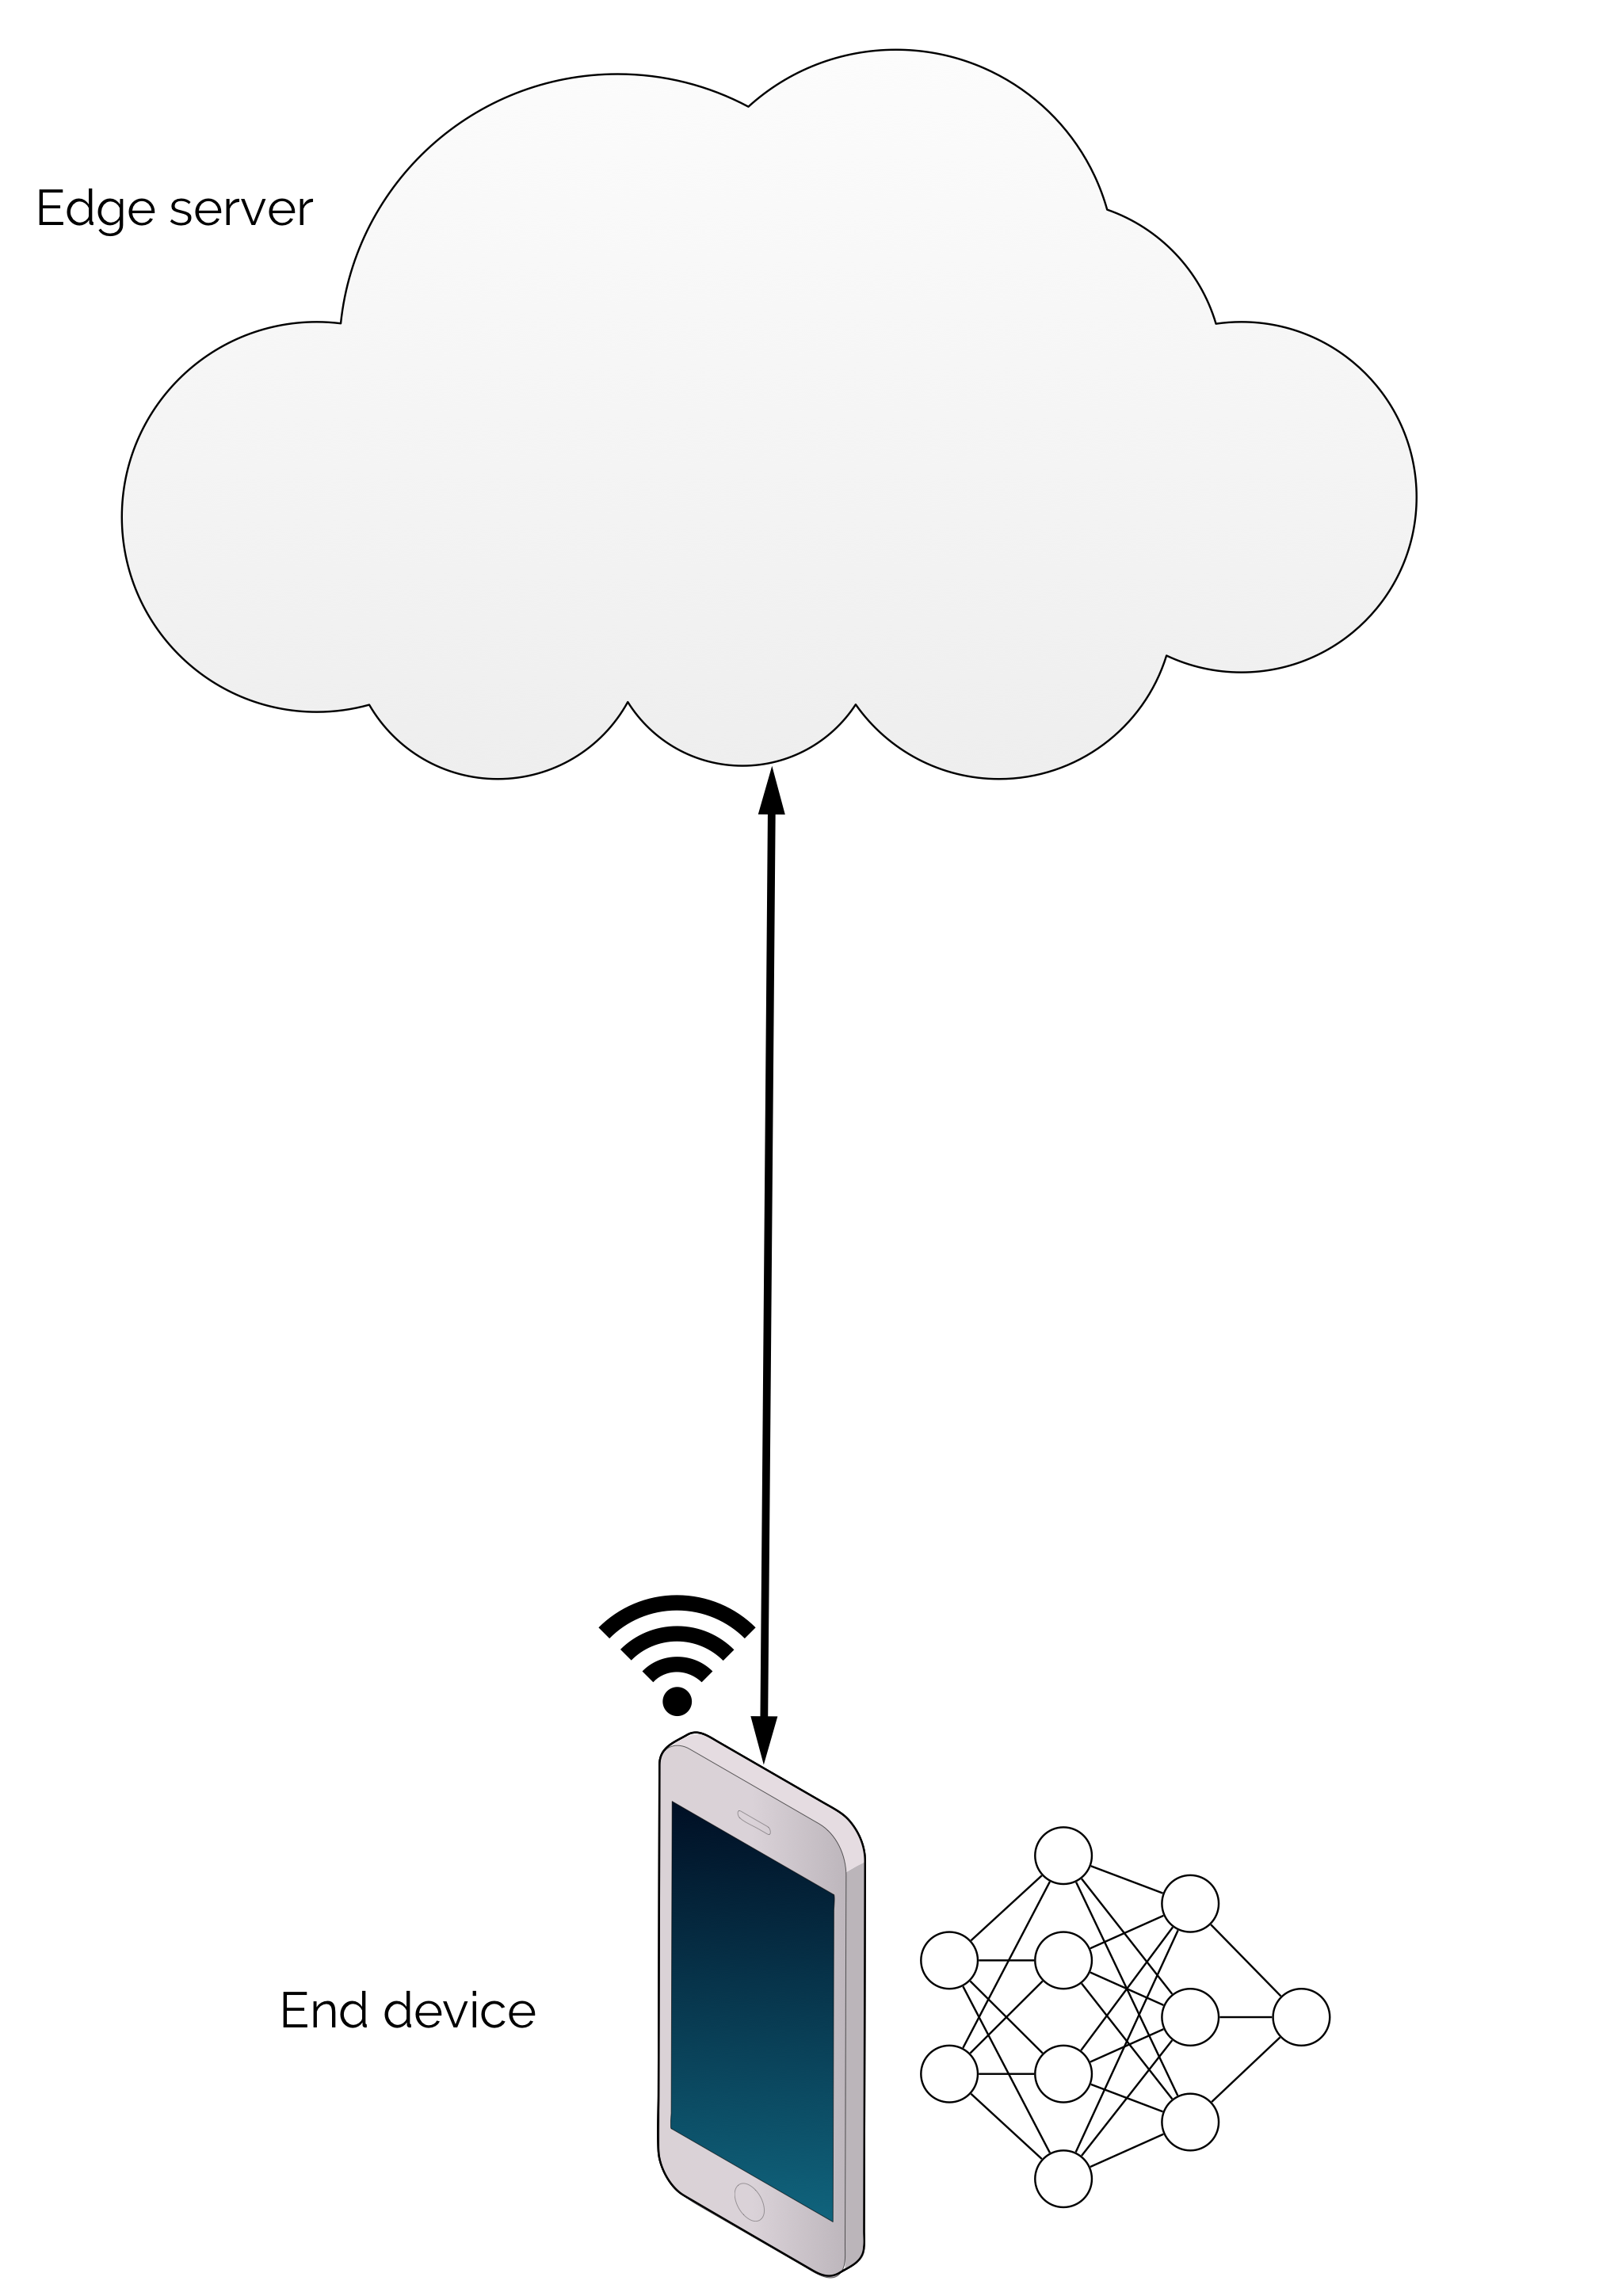
\includegraphics[width=\linewidth]{figures/models/device}}
		\end{figure}
	\end{minipage}
	
	\begin{minipage}{0.3\linewidth}
		\centering
		\begin{figure}
			\centering
			\captionsetup[subfigure]{justification=centering}
			\subfloat[Edge Offloading\label{fig:edge-based}]{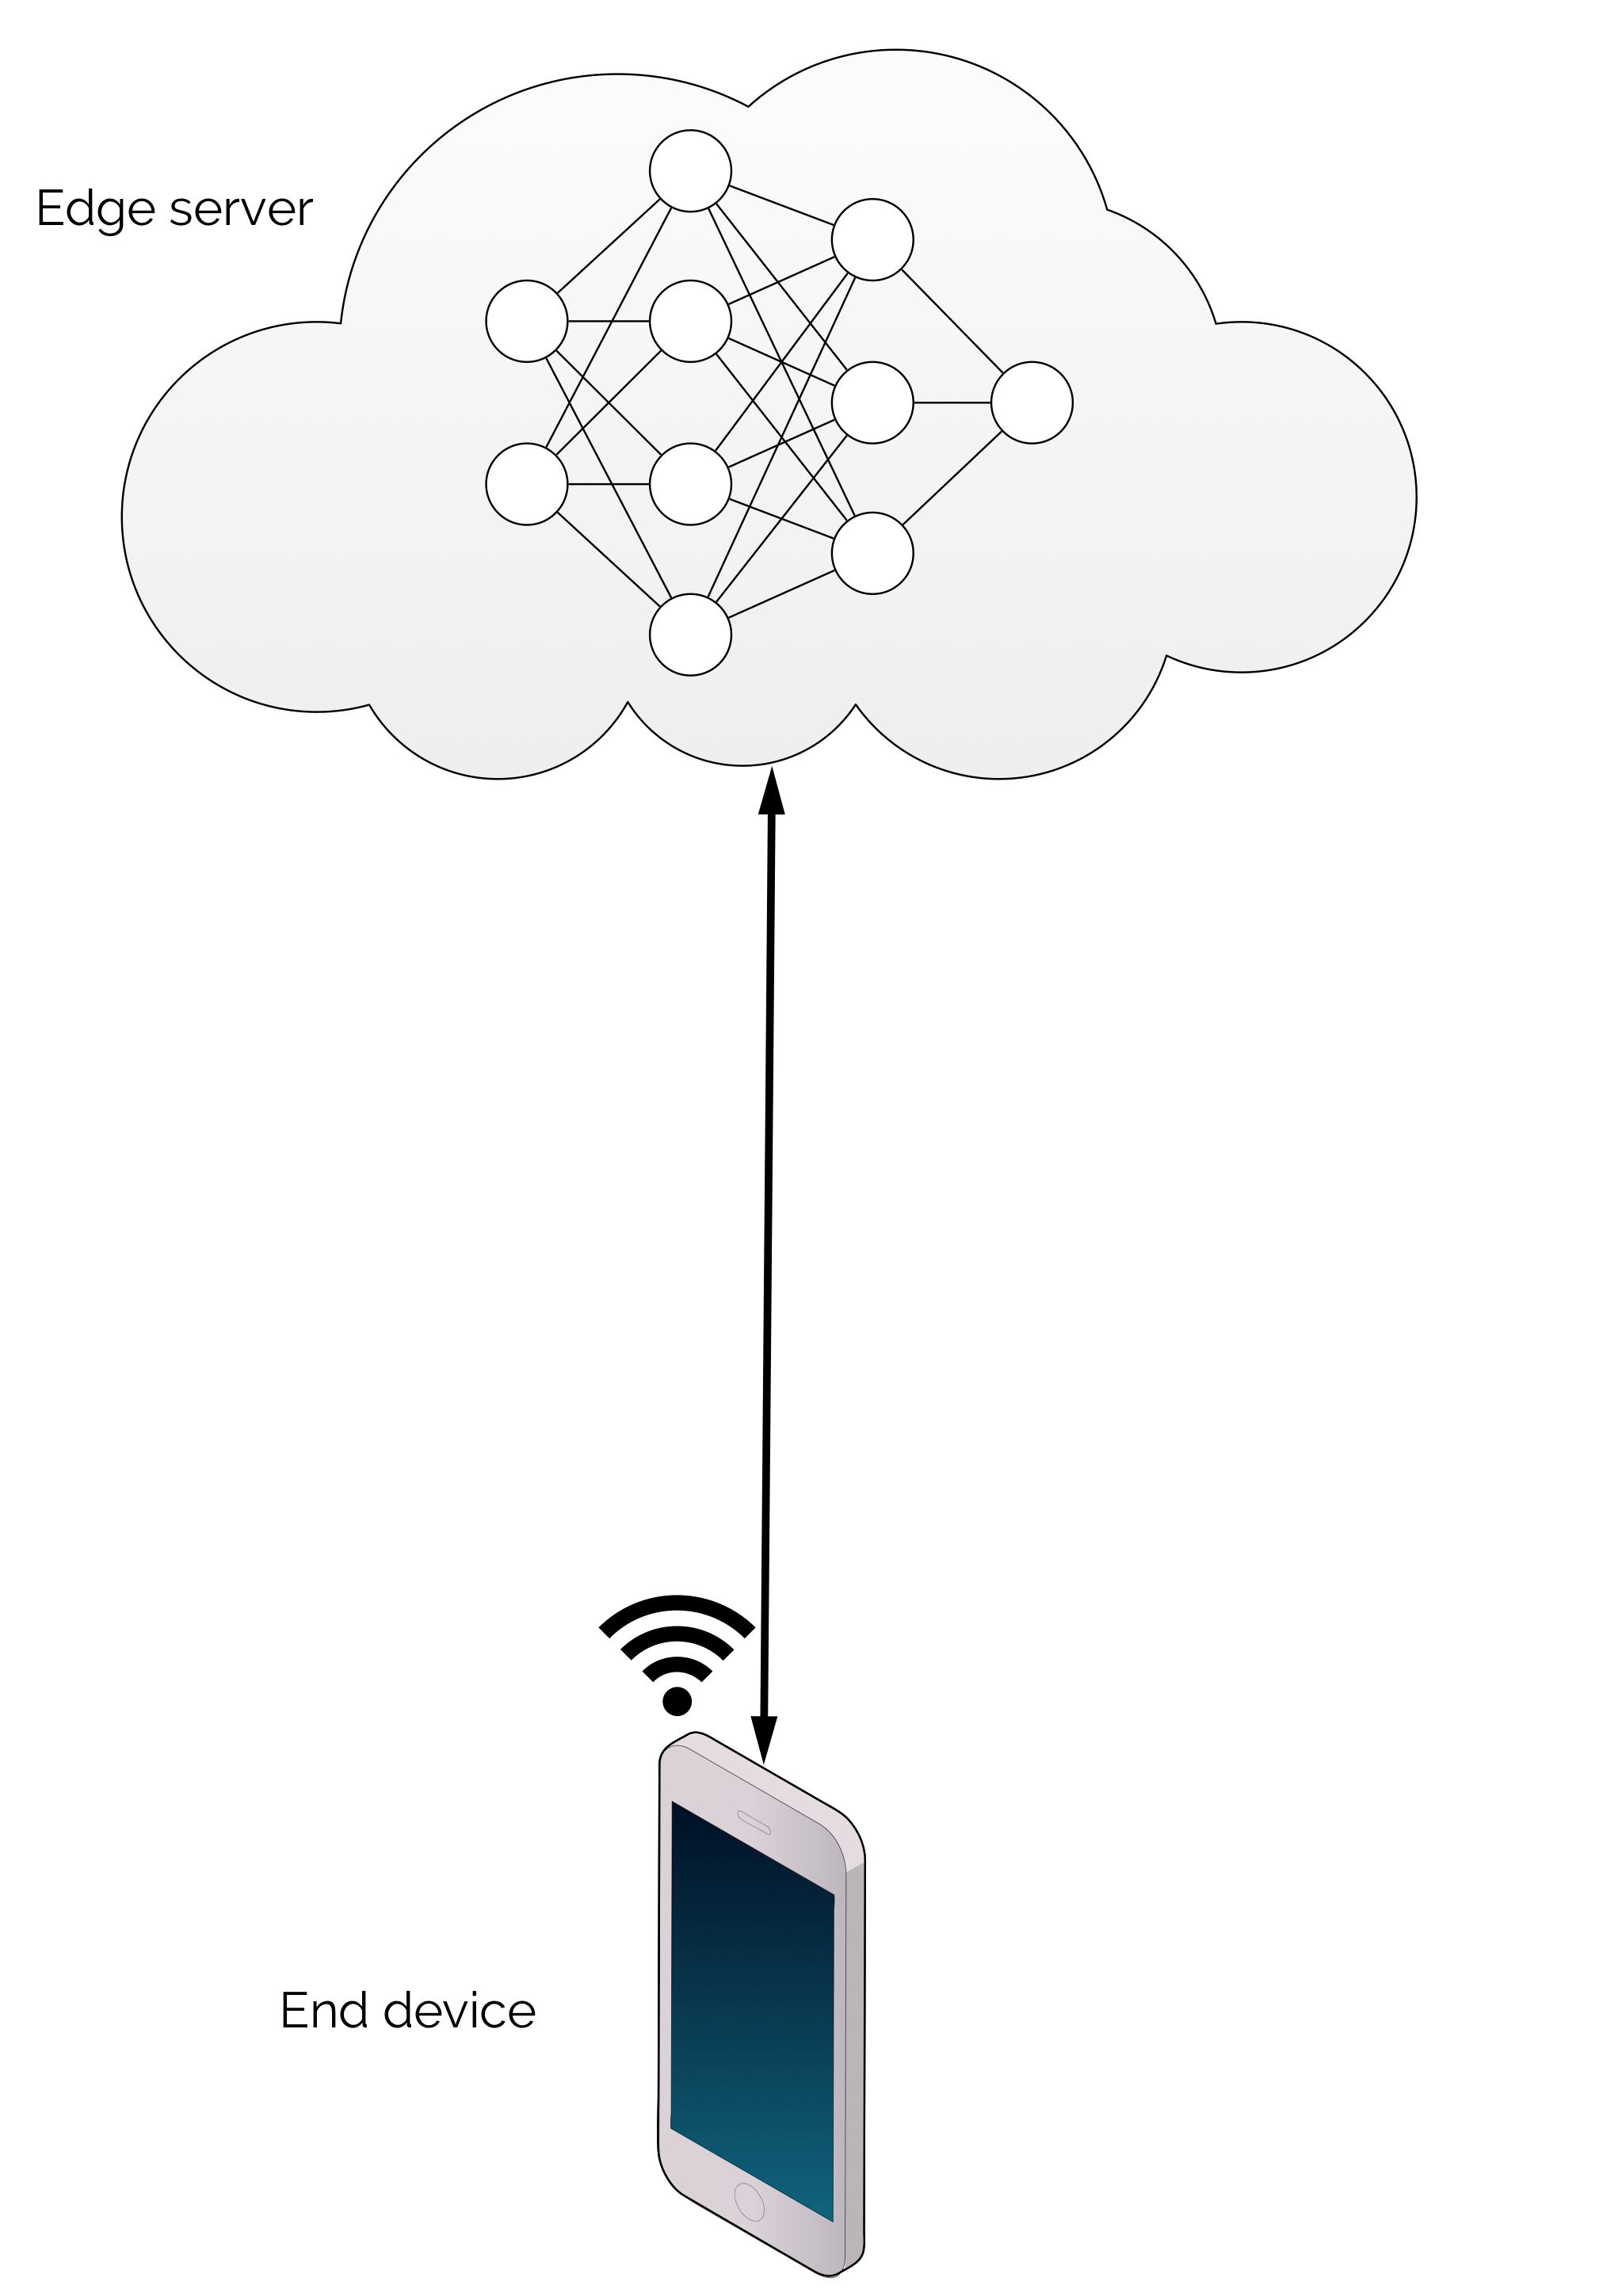
\includegraphics[width=\linewidth]{figures/models/edge}}
		\end{figure}
	\end{minipage}
	\hfill
	\begin{minipage}{0.65\linewidth}
		\textbf{\protect\subref{fig:edge-based} \textsc{Edge Infernce Offloading}}
		\color{caption-color} \newline
		Data and model inference is offloaded to the edge. The end device still acquires input data and transfer it to the edge. The edge performs model inference and send back the prediction result to the end device. The performance now relies on edge server computing resources and the available network bandwidth between end device and edge server. If time is the main concern, remote offloading is only sensible, whenever time could be saved, compared to device-based model inference. Or if energy efficiency is the main concern, remote offloading is only sensible, if energy could be saved by communicating the data to the edge.
	\end{minipage}
\end{figure}

\begin{figure}
	\begin{minipage}{0.65\linewidth}
		\textbf{\protect\subref{fig:edge-device-mode} \textsc{Collaborative Edge}}
		\color{caption-color} \newline
		The end device acquires input data and performs partial model inference. The intermediate data is transferred to an edge server which finalizes model inference. The performance relies on the computing resource of both the end device and the edge server and edge server workload, as well as, available network bandwidth between end device and edge server. Collaborative egde promotes privacy, as intermediate data of model inference is offloaded. These intermediate features have no apparent meaning for humans, which will improve the confidentiality of data.   
	\end{minipage}%
	\hfill
	\begin{minipage}{0.3\linewidth}
		\centering
		\captionsetup[subfigure]{justification=centering}
		\begin{figure}
			\centering
			\subfloat[Collaborative Edge Inference\label{fig:edge-device-mode}]{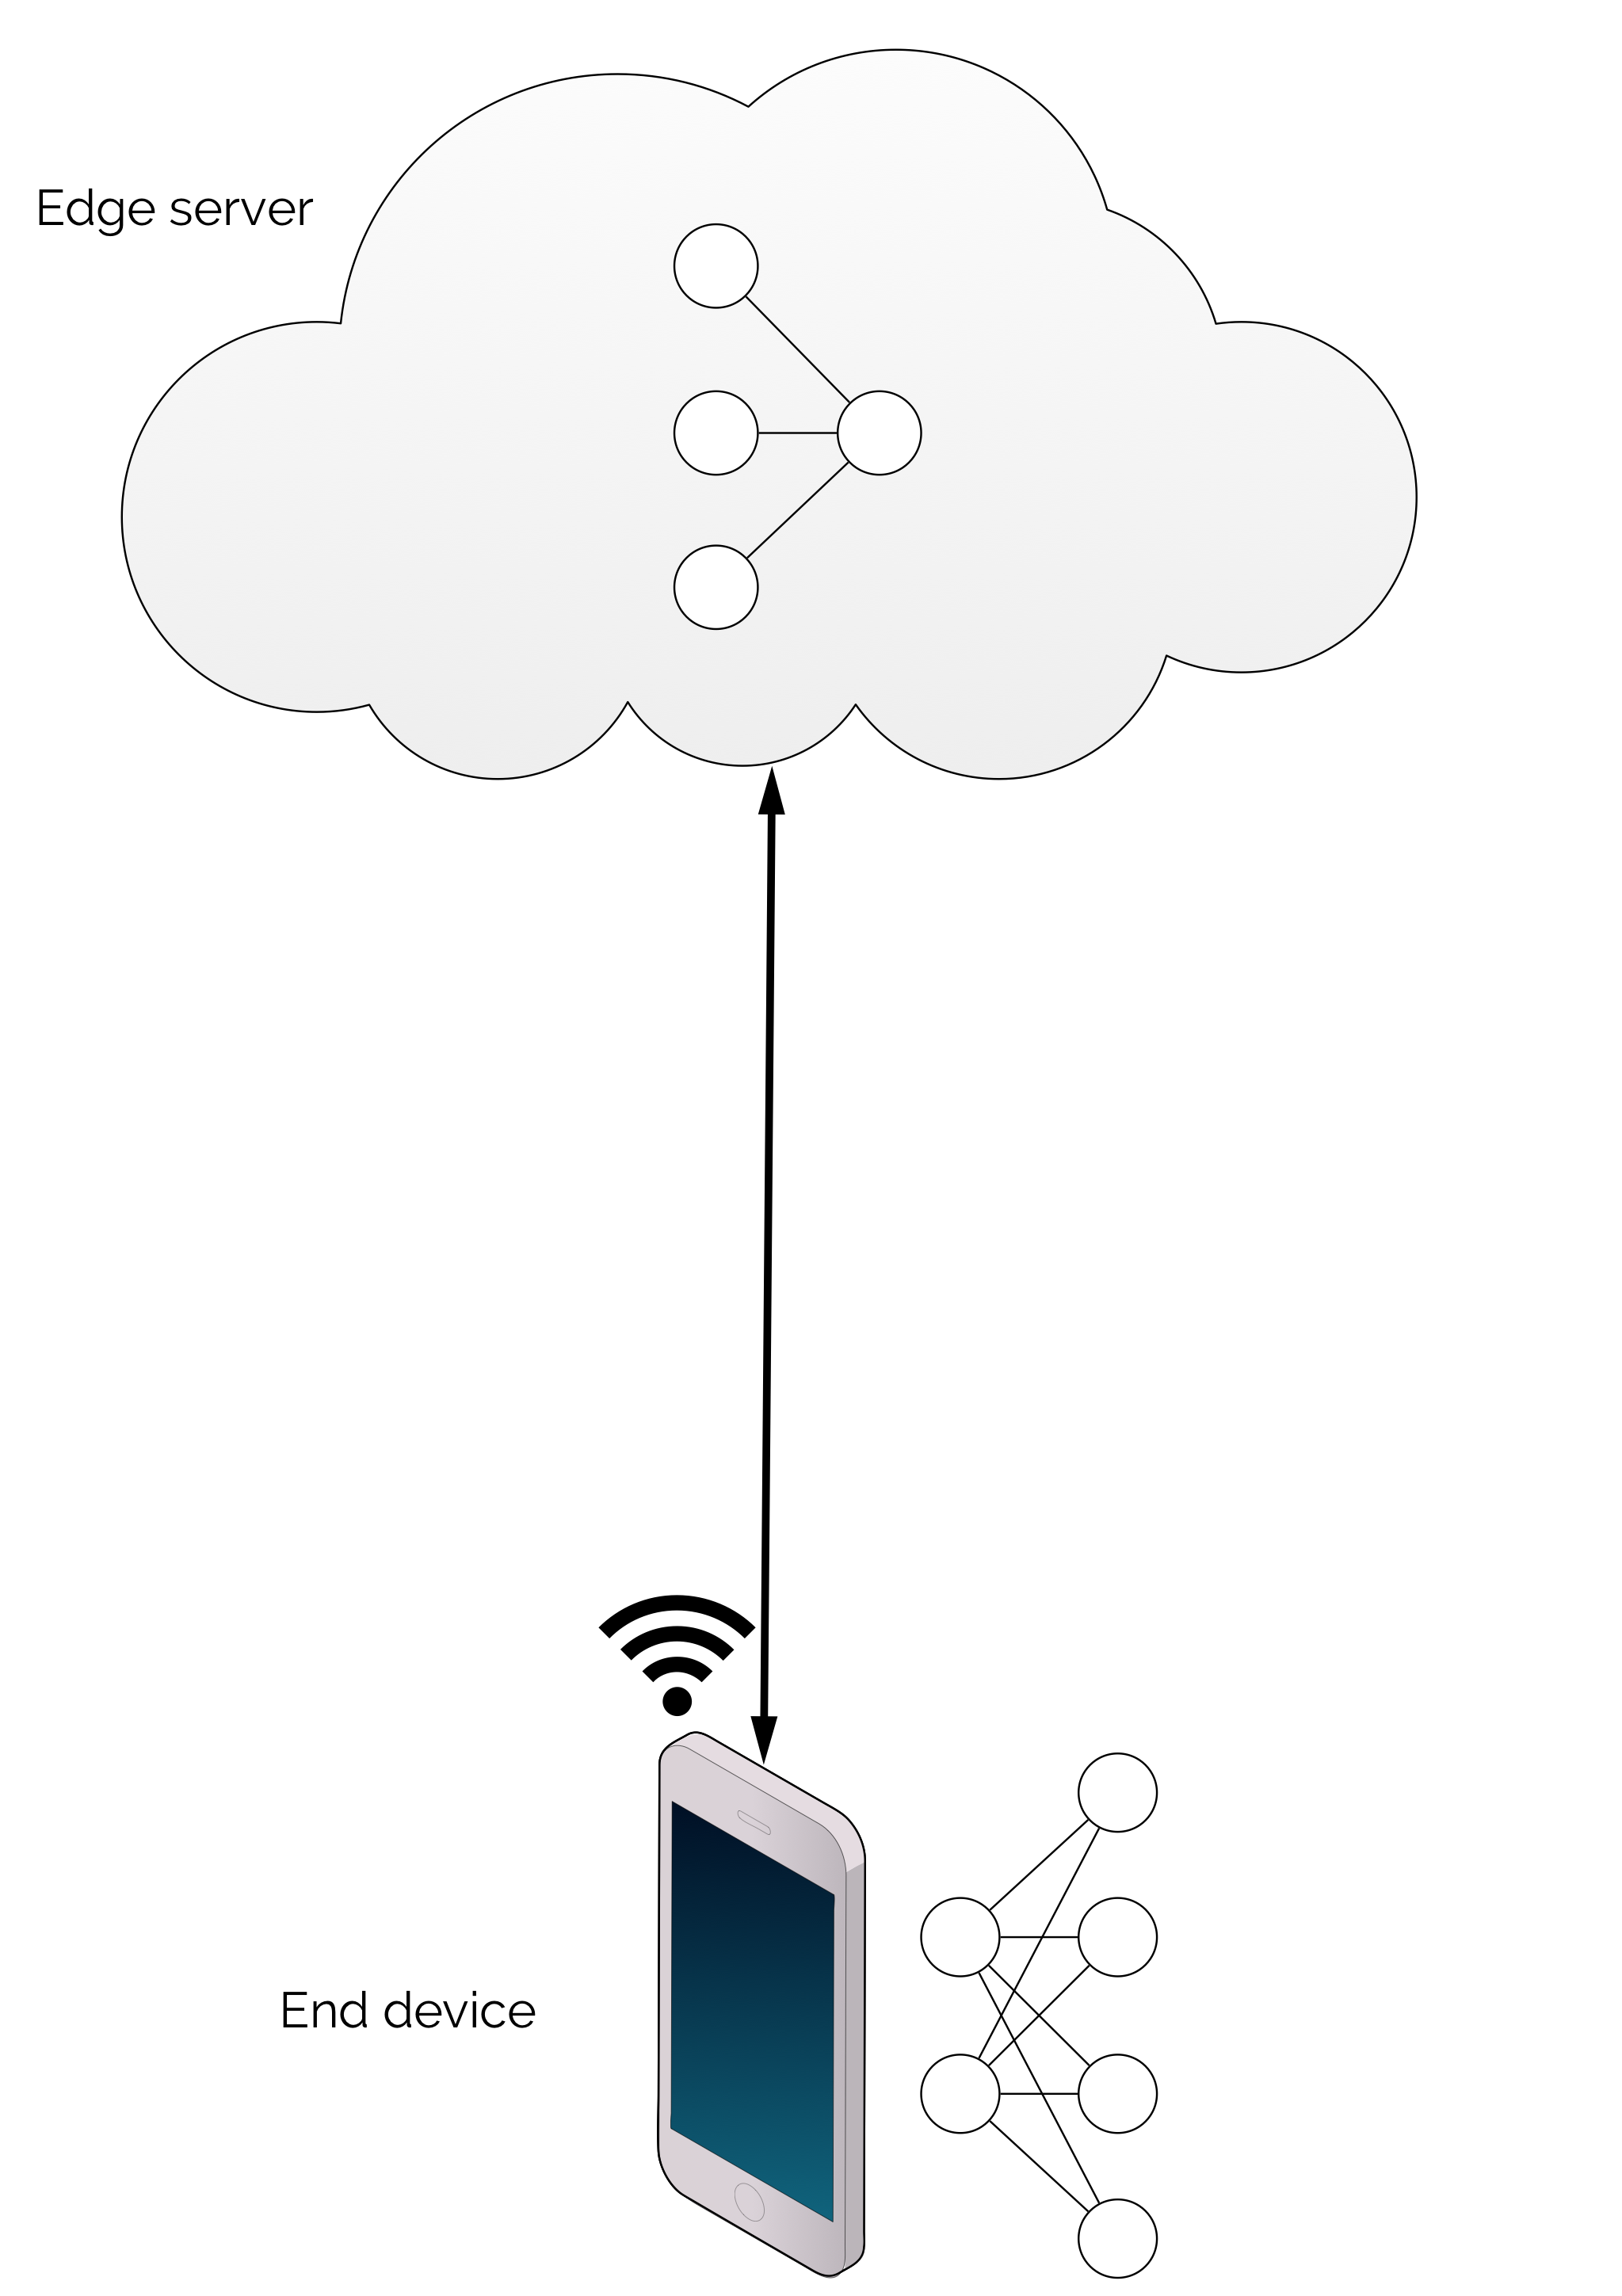
\includegraphics[width=\linewidth]{figures/models/edge_device}}
		\end{figure}
	\end{minipage}
	\begin{minipage}{0.5\linewidth}
		\centering
		\captionsetup[subfigure]{justification=centering}
		\begin{figure}
			\centering
			\subfloat[Collaborative Edge-Cloud Inference\label{fig:edge-cloud-mode}]{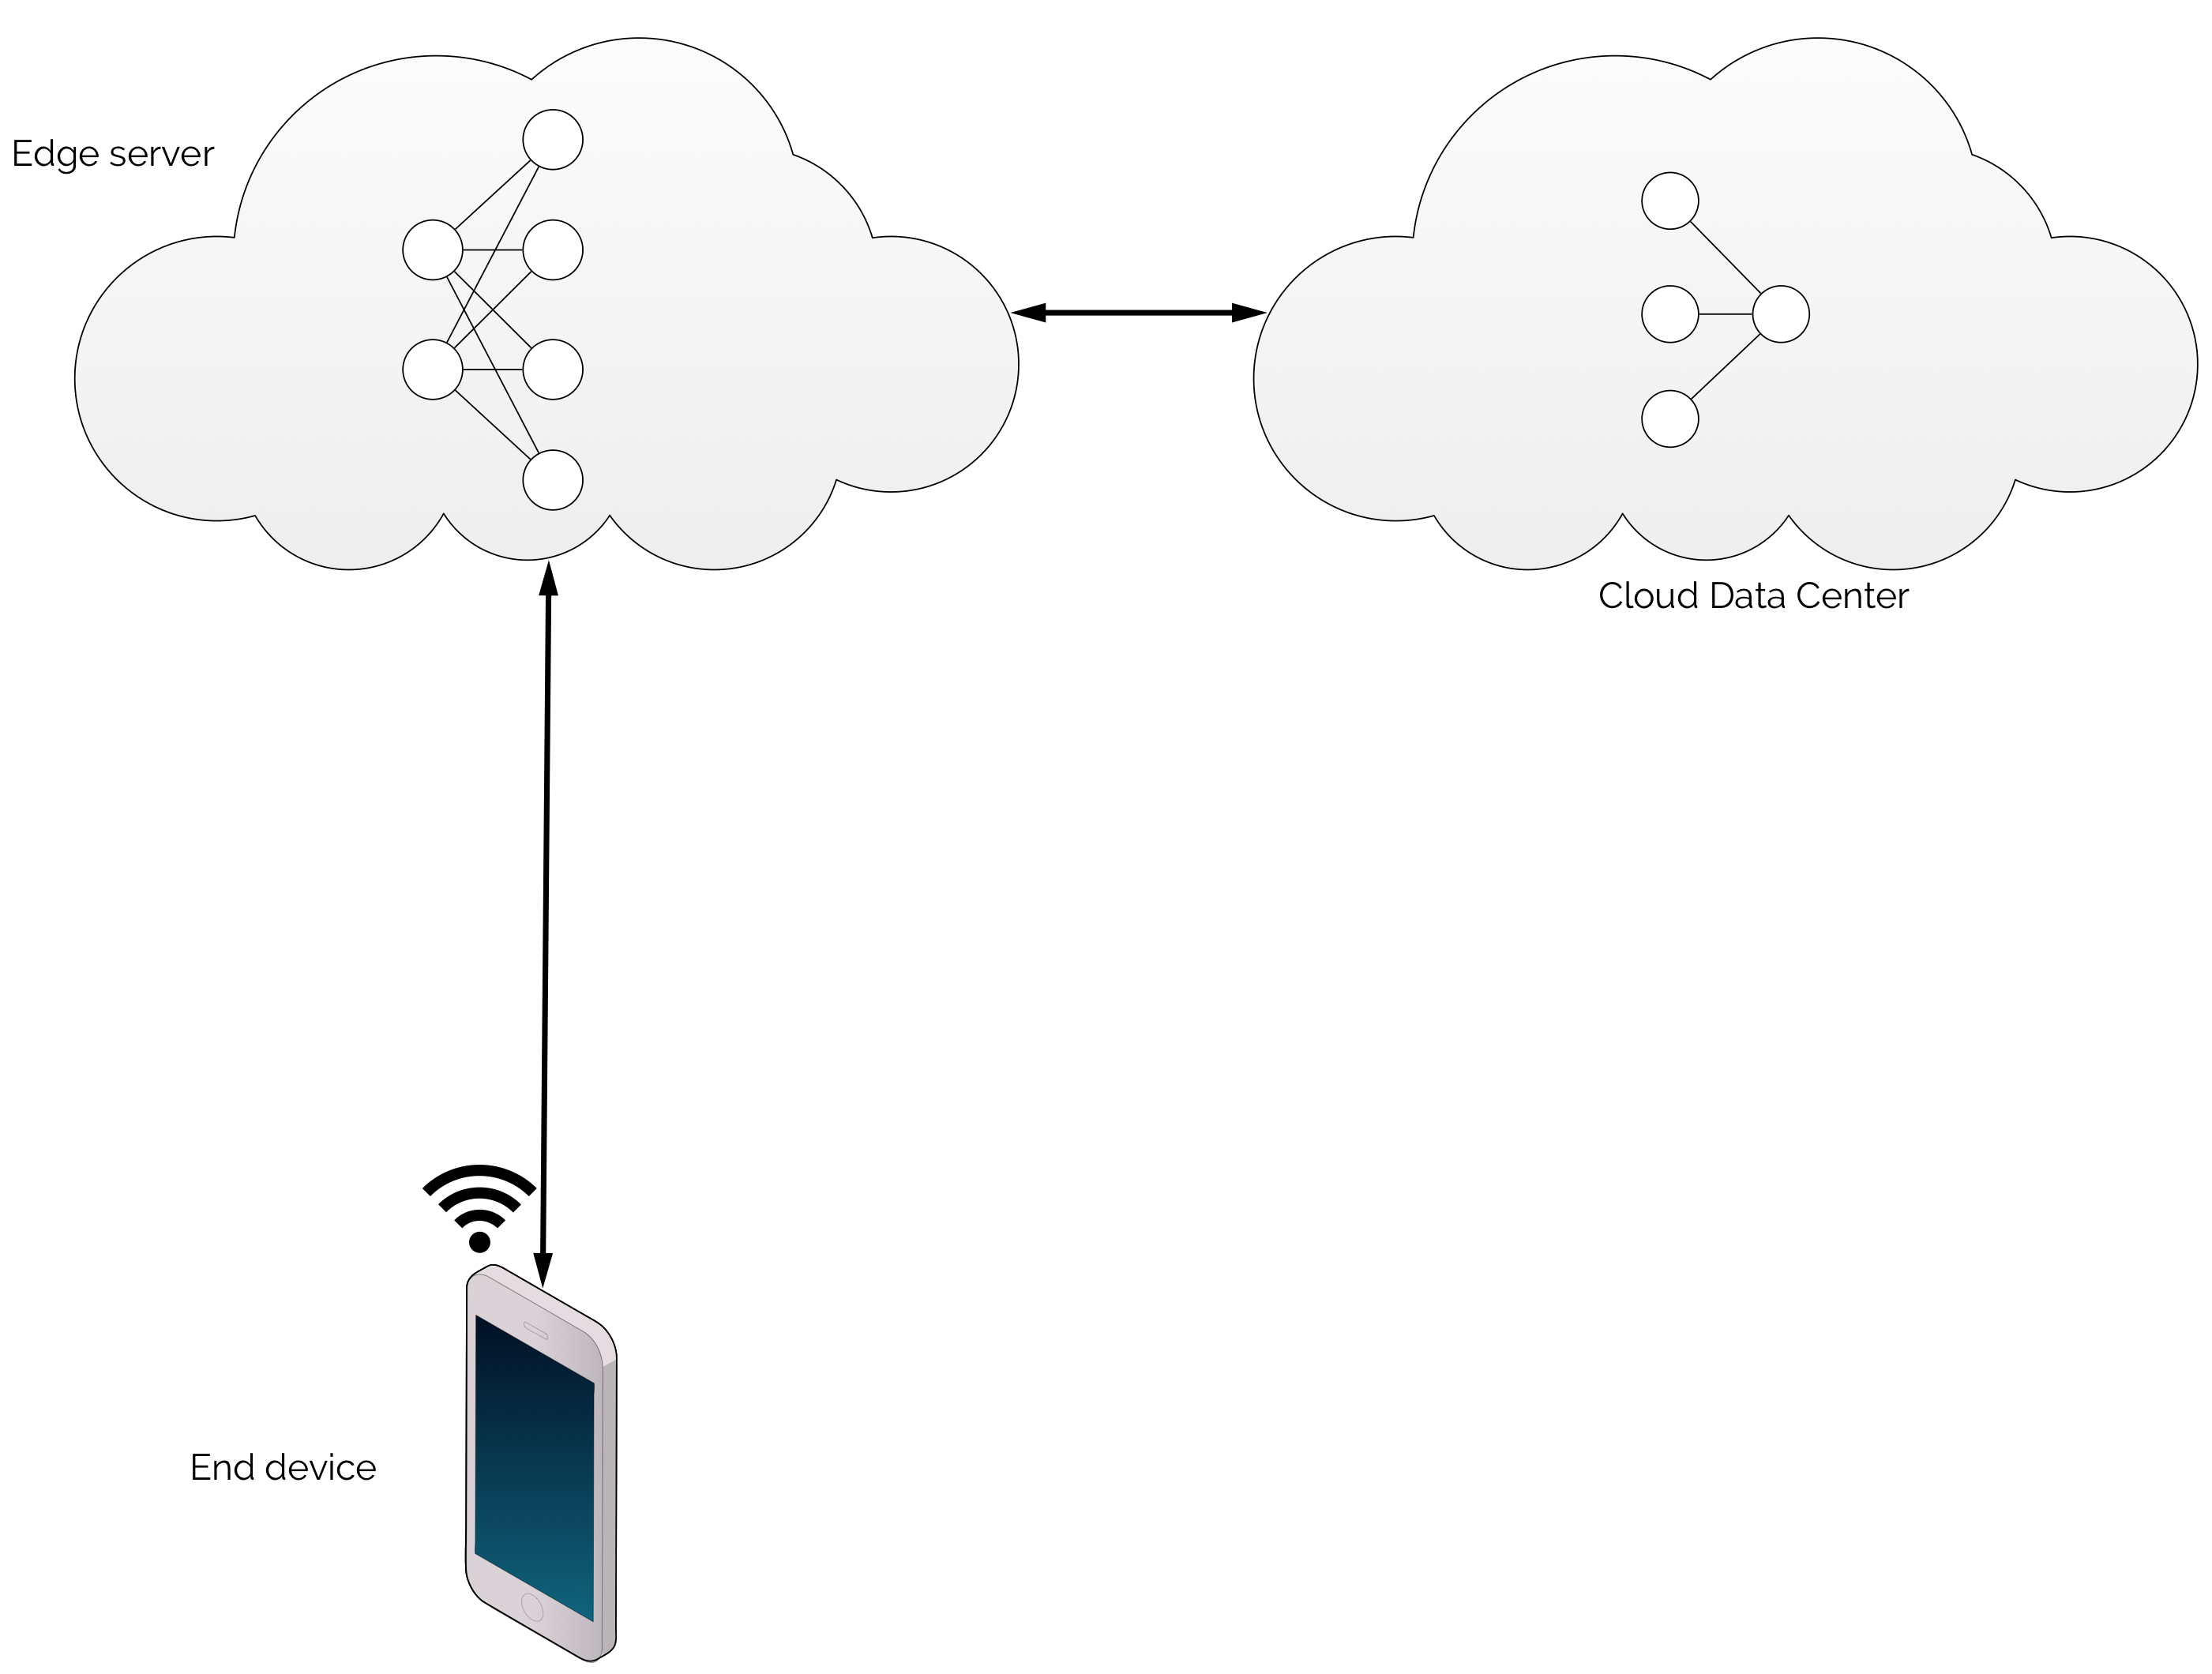
\includegraphics[width=\linewidth]{figures/models/edge_cloud}}
		\end{figure}
	\end{minipage}
	\hfill
	\begin{minipage}{0.45\linewidth}
		\textbf{\protect\subref{fig:edge-cloud-mode} \textsc{Collaborative Edge-Cloud}}
		\color{caption-color} \newline
		Resembles edge-device mode, however the model inference task is now partitioned between edge server and cloud data centers. The inference now relies on edge server's and data center's computing resources, but not least on network connection between edge and cloud. The scheme does too promote privacy, however only between edge and cloud and not in the local network at the edge. The two schemes could easily be combined to split inference between device, edge and cloud.
	\end{minipage}
	\caption[Edge-centric Architectures]{Edge-centric Architectures: \protect\subref{fig:device-based} device only execution, \protect\subref{fig:edge-based} edge only execution,\protect\subref{fig:edge-device-mode} edge and device partial execution, \protect\subref{fig:edge-cloud-mode} edge and cloud partial execution}
	\label{fig:edge_arch}
\end{figure}

The first two modes are the conventional schemes, which resembles the current \gls{di} and \gls{ci} frameworks, where all processing are done by one peer. The next two schemes presents collaborative architectures, where processing is divided for partial execution between the peers.
Moving model inference away from data centers with high-end specialized hardware offering tremendous amounts of computing power, to less powerful edge clusters or even just a single edge server. To adapt the diverse hardware landscape at the edge calls research in improvements of model inference. In the next section, we present existing literature proposals of enabling technologies aiming at reducing the model inference time.

\section{Fast Inference} \label{sec:ei-fast-inference}

In this section enabling technologies for fast inference will be described. Despite research in parallelism for \gls{cpu}s and \gls{gpu}s, efforts have been made in developing \gls{asic} or \gls{fpga}, i.e. specialized hardware such as Google's \gls{tpu} to further accelerate training and inferencing \gls{dnn}s, our main concern is model inference for real-time applications. We present efforts in literature, that operate on a model level e.g., model desing, -compression, -selection, -early exit and -layer skipping. We review literature for collaborative inference by splitting the \gls{dnn}s, such as feature compression to reduce communication delay. Additionally, we present, how model level methods can be used in collaborative edge. Table \ref{tbl:fast-inference} summarizes the technologies, which is explained in greater detail in this section. We omit technologies that operates on a infrastructural level e.g., edge caching, input filtering and support for multi-tenancy \cite{zhou_edge_2019}.
\begin{minipage}[t]{\linewidth}
\begin{tiny}
\begin{longtabu}{>{\bfseries}X[0.8c]|X[c]|X[c]|X[c]|X[c]|X[c]}
	\caption[Fast Inference Related Work]{Fast inference related work categorized by architecture and technology. On device and edge offloading have been collapsed, as the only difference between the two is the additional communication of data to offload the inference task to the edge. Collaborative edge and edge cloud are collapsed, as the methods apply to both and only depends on infrastructure.} \label{tbl:fast-inference} \\
	\toprule
	\rowfont{\bfseries}
	Architecture & Technology & Speed-Up method & Advantages & Disadvantages & Works \tabularnewline
	\hline
	\endfirsthead
	\multicolumn{3}{@{}l}{\textbf{\textcolor{black}{Table \ref{tbl:fast-inference}:}} continued}\\
	\toprule
	\rowfont{\bfseries}
	Architecture & Technology & Speed-Up method & Advantages & Disadvantages & Works \tabularnewline
	\hline
	\endhead % all the lines above this will be repeated on every page
	\hline
	\multicolumn{3}{@{}l}{continued \ldots}\\
	\endfoot
	\hline
	\endlastfoot
	 \multirow{5}{*}{\rotatebox[origin=c]{90}{\parbox[c]{4cm}{On-Device or Edge Offloading}}} & Model Design & Innovative layer and operation design & Combineable, Reduce Memory footprint  & Accuracy cost & \cite{iandola_squeezenet:_2016,howard_mobilenets:_2017,sandler_mobilenetv2:_2018, zhang_shufflenet:_2017, ma_shufflenet_2018} \tabularnewline
	\tabucline{2-6}
	
	& Model Compression & Reduce model size & Adaptive, Combineable, Reduce Memory footprint & Accuracy cost &  \cite{hinton_distilling_2015,courbariaux_binaryconnect:_2015,courbariaux_binarized_2016,romero_fitnets:_2014} \tabularnewline	
	& & & & & \tabularnewline
	\tabucline{2-6}
	
	& Model Selection & Reduce depth overhead by selecting smaller model & Adaptive, Early exit & Accuracy cost, may require multiple \gls{dnn} inferences & \cite{bolukbasi_adaptive_2017, tann_flexible_2018, park_big/little_2015} \tabularnewline
	\tabucline{2-6}
	
	& Model Early Exit & Reduce depth overhead using less layers & Adaptive, Early exit, No additional inference, Multiple predictions & Accuracy cost, Possible lack of coarse level features & \cite{leroux_resource-constrained_2015,teerapittayanon_branchynet:_2016, berestizshevsky_sacrificing_2019, kaya_shallow-deep_nodate, huang_multi-scale_2017} \tabularnewline
	\tabucline{2-6}
	& Model Layer Skipping & Reduce depth overhead using less layers & Adaptive, Coarse level features & Accuracy cost, require additional reinforcement learning of skipping policies & \cite{wang_skipnet:_2017,wu_blockdrop:_2017} \tabularnewline\hline
		
	\multirow{2}{*}{\rotatebox[origin=c]{90}{\parbox[c]{2.2cm}{Collaborative Edge\\ or Edge-Cloud}}} & Feature Compression & Reduce size of intermediate feature size to reduce communication latency & Utilize a more powerful device for heavy processing  & Accuracy cost, Compression aware training, compression time & \cite{kang_neurosurgeon:_2017,choi_near-lossless_2018, choi_deep_2018, eshratifar_bottlenet:_2019} \tabularnewline
 	\tabucline{2-6}
	
	& Distributed Exits & Reduced depth and communication overhead of offloading using local exits  &  Reduce unnecessary communication efforts, same inference task & Accuracy cost, computation latency overhead from local processing, communication latency if not exiting locally & \cite{leroux_cascading_2017,teerapittayanon_distributed_2017, li_edge_2018} \tabularnewline\hline
	
	\rotatebox[origin=r]{90}{Distributed} & Input-wise partitioning & Distributing workload to multiple peers & Constraint devices, which could not solely run inference, can collaborate to solve the task & Orchestration, Synchronization, Data dependence between peers & \cite{mao_modnn:_2017, zhao_deepthings:_2018}
	\tabularnewline

	\bottomrule
\end{longtabu}
\end{tiny}
\end{minipage}

\subsection{On-device or Edge Offloading}

In this subsection efforts to reduce inference time for on-device or edge offloading \gls{dnn}s are presented.

\begin{enumdescript}
	\item[Model Design] To improve inference latency efforts have been made in designing \gls{dnn}s, that reduces the size of the model, thus reducing the memory footprint to run more efficiently on mobile and \gls{iot} devices. Most efforts addresses ways to reduce the number of parameters, such as \gls{squeezenet} \cite{iandola_squeezenet:_2016} down samples the data size using convolutions. Or by creating more efficient models, that reduces the amount of \acrshort{flop}s required for the model. \gls{mobilenet}s \cite{howard_mobilenets:_2017,sandler_mobilenetv2:_2018} decomposes the convolution filters into simpler operations, thus reduces the amount of computations for the model. \gls{shufflenet}s \cite{zhang_shufflenet:_2017, ma_shufflenet_2018}, that uses a point-wise convolution operation and channel shuffling to reduce the amount of computations. Other efforts have been made to reduce the number of parameters for existing \gls{dnn} architectures using model compression.
	
	\item[Model compression]  is about finding a more compact or compressed way to represent the model. Pruning is probably the most widespread compression technique. Pruning can be used to create sparse networks, by removing the least contributing neurons and connections. Pruning have shown significant speed-ups with only a small loss in accuracy \cite{zhou_edge_2019}. The impact of compression is application dependent and can be applied to any pre-trained \gls{dnn} and in combination with other techniques \cite{cheng_survey_2017}.
	
	\begin{minipage}[t]{\linewidth}
		\centering
		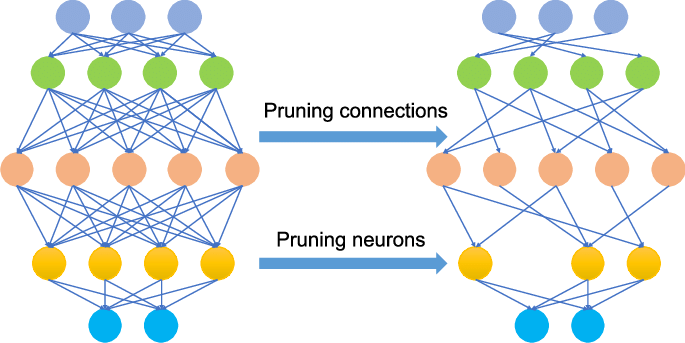
\includegraphics[width=.4\linewidth]{figures/articles/Pruning-a-neural-network}
		\captionof{figure}[\gls{dnn} Pruning]{Pruning conection and neurons source: \citetitle{chen_deep_2019} \cite{chen_deep_2019}}
	\end{minipage}
	
	Another compression technique is quantization. A more compact representation of weights are used to reduce the amount of bits needed for each weight of the model \cite{cheng_survey_2017}. The extreme case is binarization, where weights and activations are learned as a binary representations. In BinaryConnect \cite{courbariaux_binaryconnect:_2015} and \gls{bnn} \cite{courbariaux_binarized_2016} most arithmetic operations are replaced with bit-wise operations, thus greatly improving the power-efficiency and inference latency. However, using binary weights in extremely deep network have also shown significant degradation of model accuracy \cite{cheng_survey_2017}.
	
	In \cite{hinton_distilling_2015} \gls{kd} has been proposed. \gls{kd} is a framework to train \gls{dnn} in a student-teacher paradigm. The student network are penalized using the output of an ensemble of teacher networks. \gls{kd} can be viewed as a compression of an ensemble of teacher network into a student network \cite{cheng_survey_2017}. 
	In \cite{romero_fitnets:_2014} \gls{fitnet} have been proposed as a method to train thinner and shallower student networks using a deeper teacher network. FitNet learns the student network to mimick the teacher network, however this approach require the softmax loss function, which limits its usage \cite{cheng_survey_2017}.  
	
	\item[Model Selection] Model selection is an approach to reduce inference by selecting an appropriately accurate model, hence not using an unnecessarily deep model, if a shallower model could give a satisfying prediction. In \cite{bolukbasi_adaptive_2017} an adaptive model selection framework is proposed. The framework stacks three \gls{dnn} with increasing depth and increasingly higher accuracy models; \gls{alexnet}, \gls{googlenet} and \gls{resnet}50. 

	\begin{minipage}[t]{\linewidth}
		\centering                           
		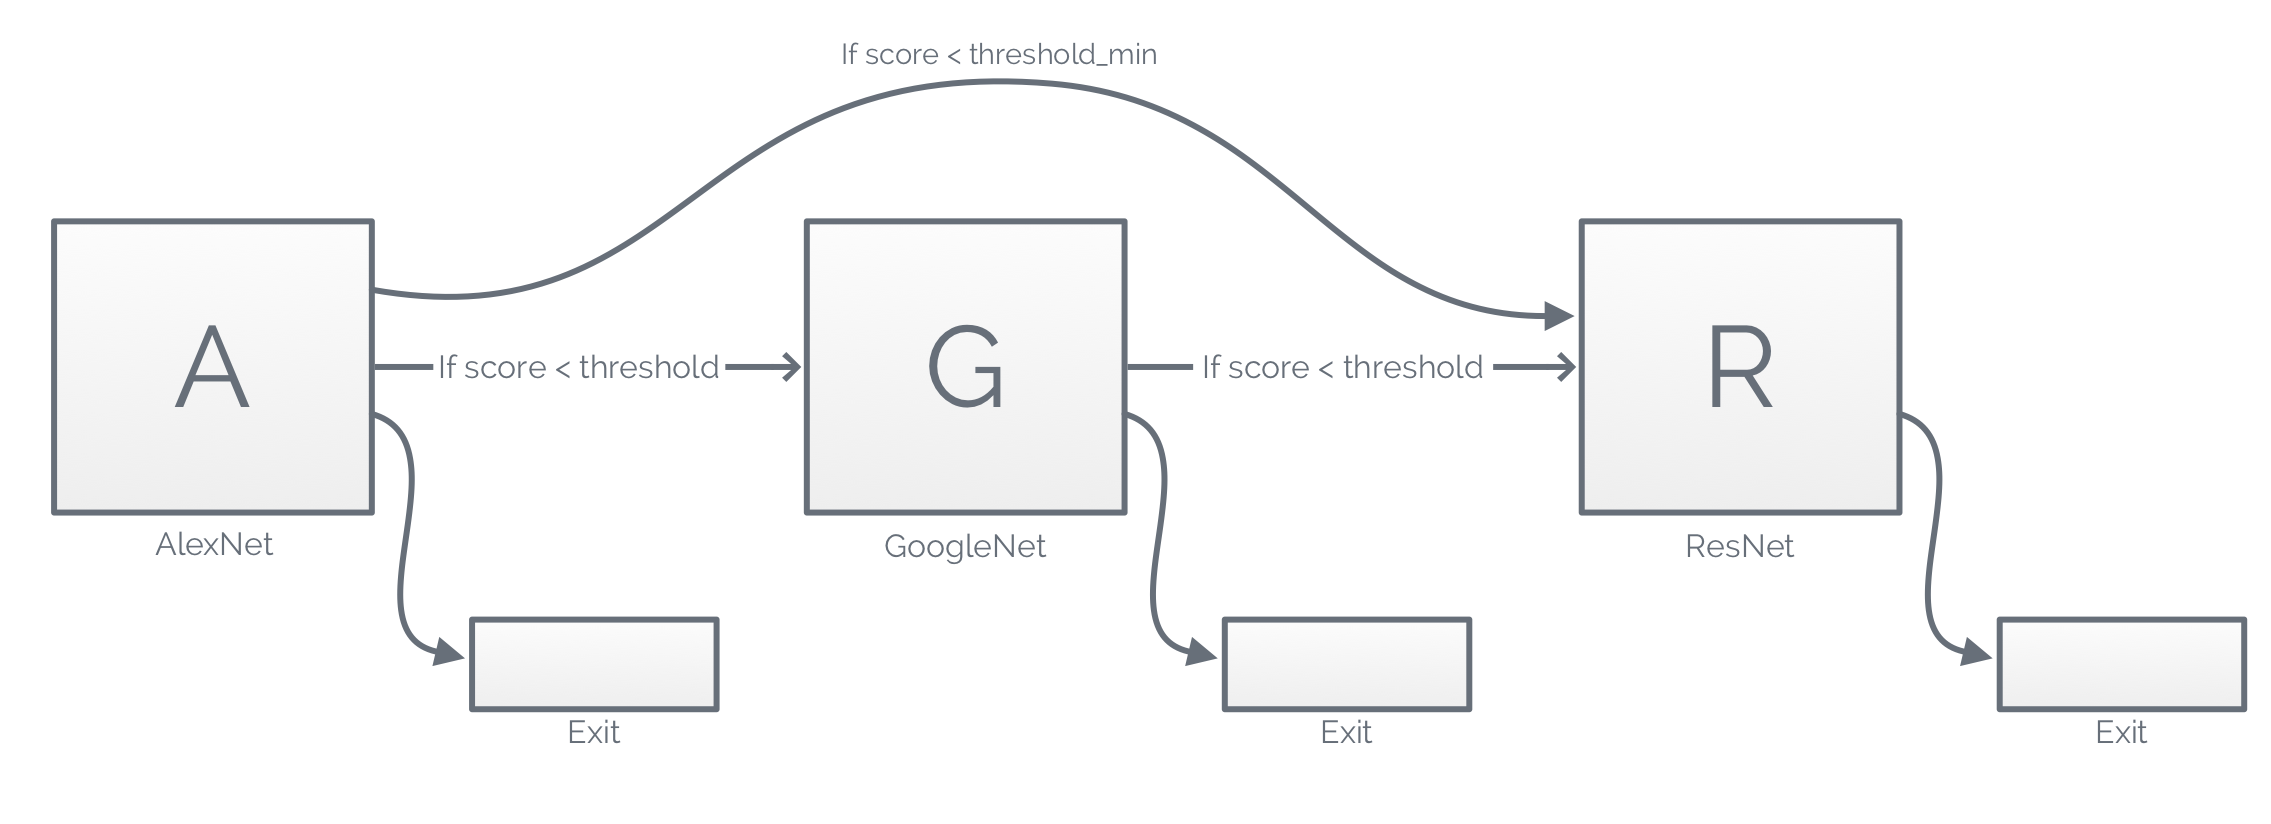
\includegraphics[width=.8\linewidth]{figures/models/adaptive}
		\captionof{figure}[Adaptive Neural Network]{Adaptive Neural Network using model selection}
	\end{minipage}
	
	The input is inferred to \gls{alexnet}, if the confidence scores is satisfying the prediction is accepted. If not the framework decides to use either \gls{googlenet} or \gls{resnet}50 depending on a confidence threshold. However, if the sample is inferred to \gls{googlenet} and the confidence is still unsatisfying the sample is inferred to \gls{resnet}50 for final prediction. In \cite{tann_flexible_2018} they propose stacking an ensemble of networks in the same manner. Both works shows improvement of the average prediction time with only a small reduction in accuracy depending on the confidence threshold. However, for hard samples, since multiple model are introduced, the inference time is increased, as well as the computational cost and memory consumption, thus such model selection approach seems overwhelming to introduce on a constraint end device. Yet it may be feasible to offload to the edge using a Big/Little setup.
	
	To obtain faster inference Big/Little \gls{dnn} \cite{park_big/little_2015} implements a hybrid architecture of device and selective offloading for edge processing. It runs a shallower, albeit less accurate model on device, and a deep and more accurate model on the edge server, as illustrated by figure \ref{fig:big/little-dnn}. 
	
	\begin{minipage}[t]{\linewidth}    
		\centering                          
		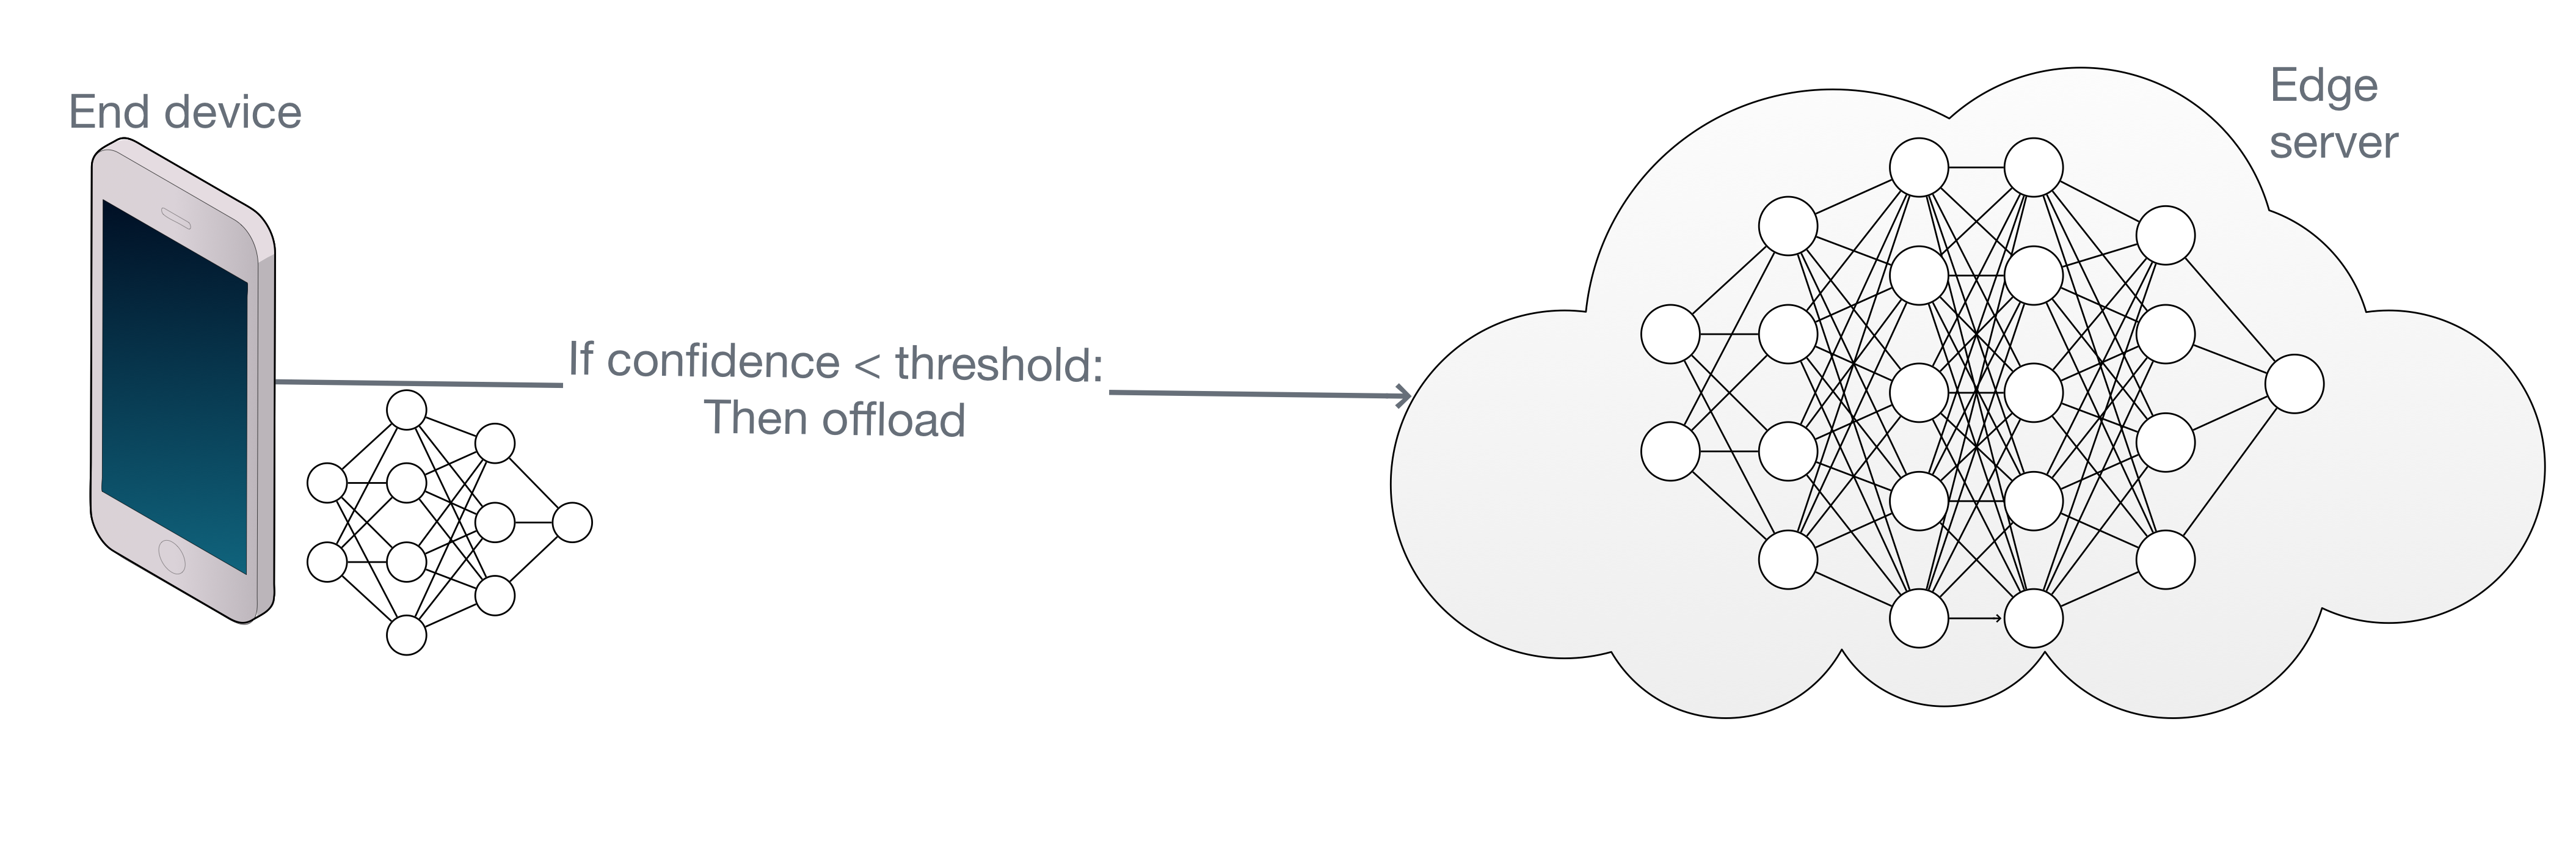
\includegraphics[width=.8\linewidth]{figures/models/big_little_dnn}
		\captionof{figure}[Big/Little \gls{dnn} architecture]{Big/Little \gls{dnn}, a hybrid edge architecture. An on-device model is used to selectively offload to a more complex model hosted on an edge server.}
		\label{fig:big/little-dnn}
	\end{minipage}
	
	If the prediction confidence of the little model is unsatisfactory, a decision is made to offload to the big model on the edge server. If a lot of samples are able to be correctly classified locally, a speed-up is gained by avoiding unnecessary communication and running a unnecessarily deep model. However, the down-side of this approach is, if too many samples require the big model to satisfy a certain confidence threshold, a lot of work is wasted on the on-device prediction. 
	
	\item[Model Early Exit] Cascading \gls{dnn} \cite{leroux_resource-constrained_2015} and \gls{branchynet} \cite{teerapittayanon_branchynet:_2016} are both early exiting frameworks for fast inference using \gls{dnn}s. Research have shown, that only a few number of samples actually require extremely deep models to be correctly classified. The frameworks, illustrated in figure \ref{fig:branchynet}, adds a cascade of intermediate classifiers, or branch exits to the \gls{dnn}, that allow samples with a higher score than a selected threshold to be classified and terminate the inference process early. Other samples may require a later exit to obtain a high enough confidence score, or perhaps the entire depth of the model. The selection of an early exit threshold resembles model selection, if a too high threshold is selected, only a few sample might be able to exit the model, thus no significant reduction in inference time is found. If too low a threshold a lot of samples will exit the model prematurely and be incorrectly classified, thus degrading the model accuracy. 

	\begin{minipage}[t]{\linewidth}    
		\centering                          
		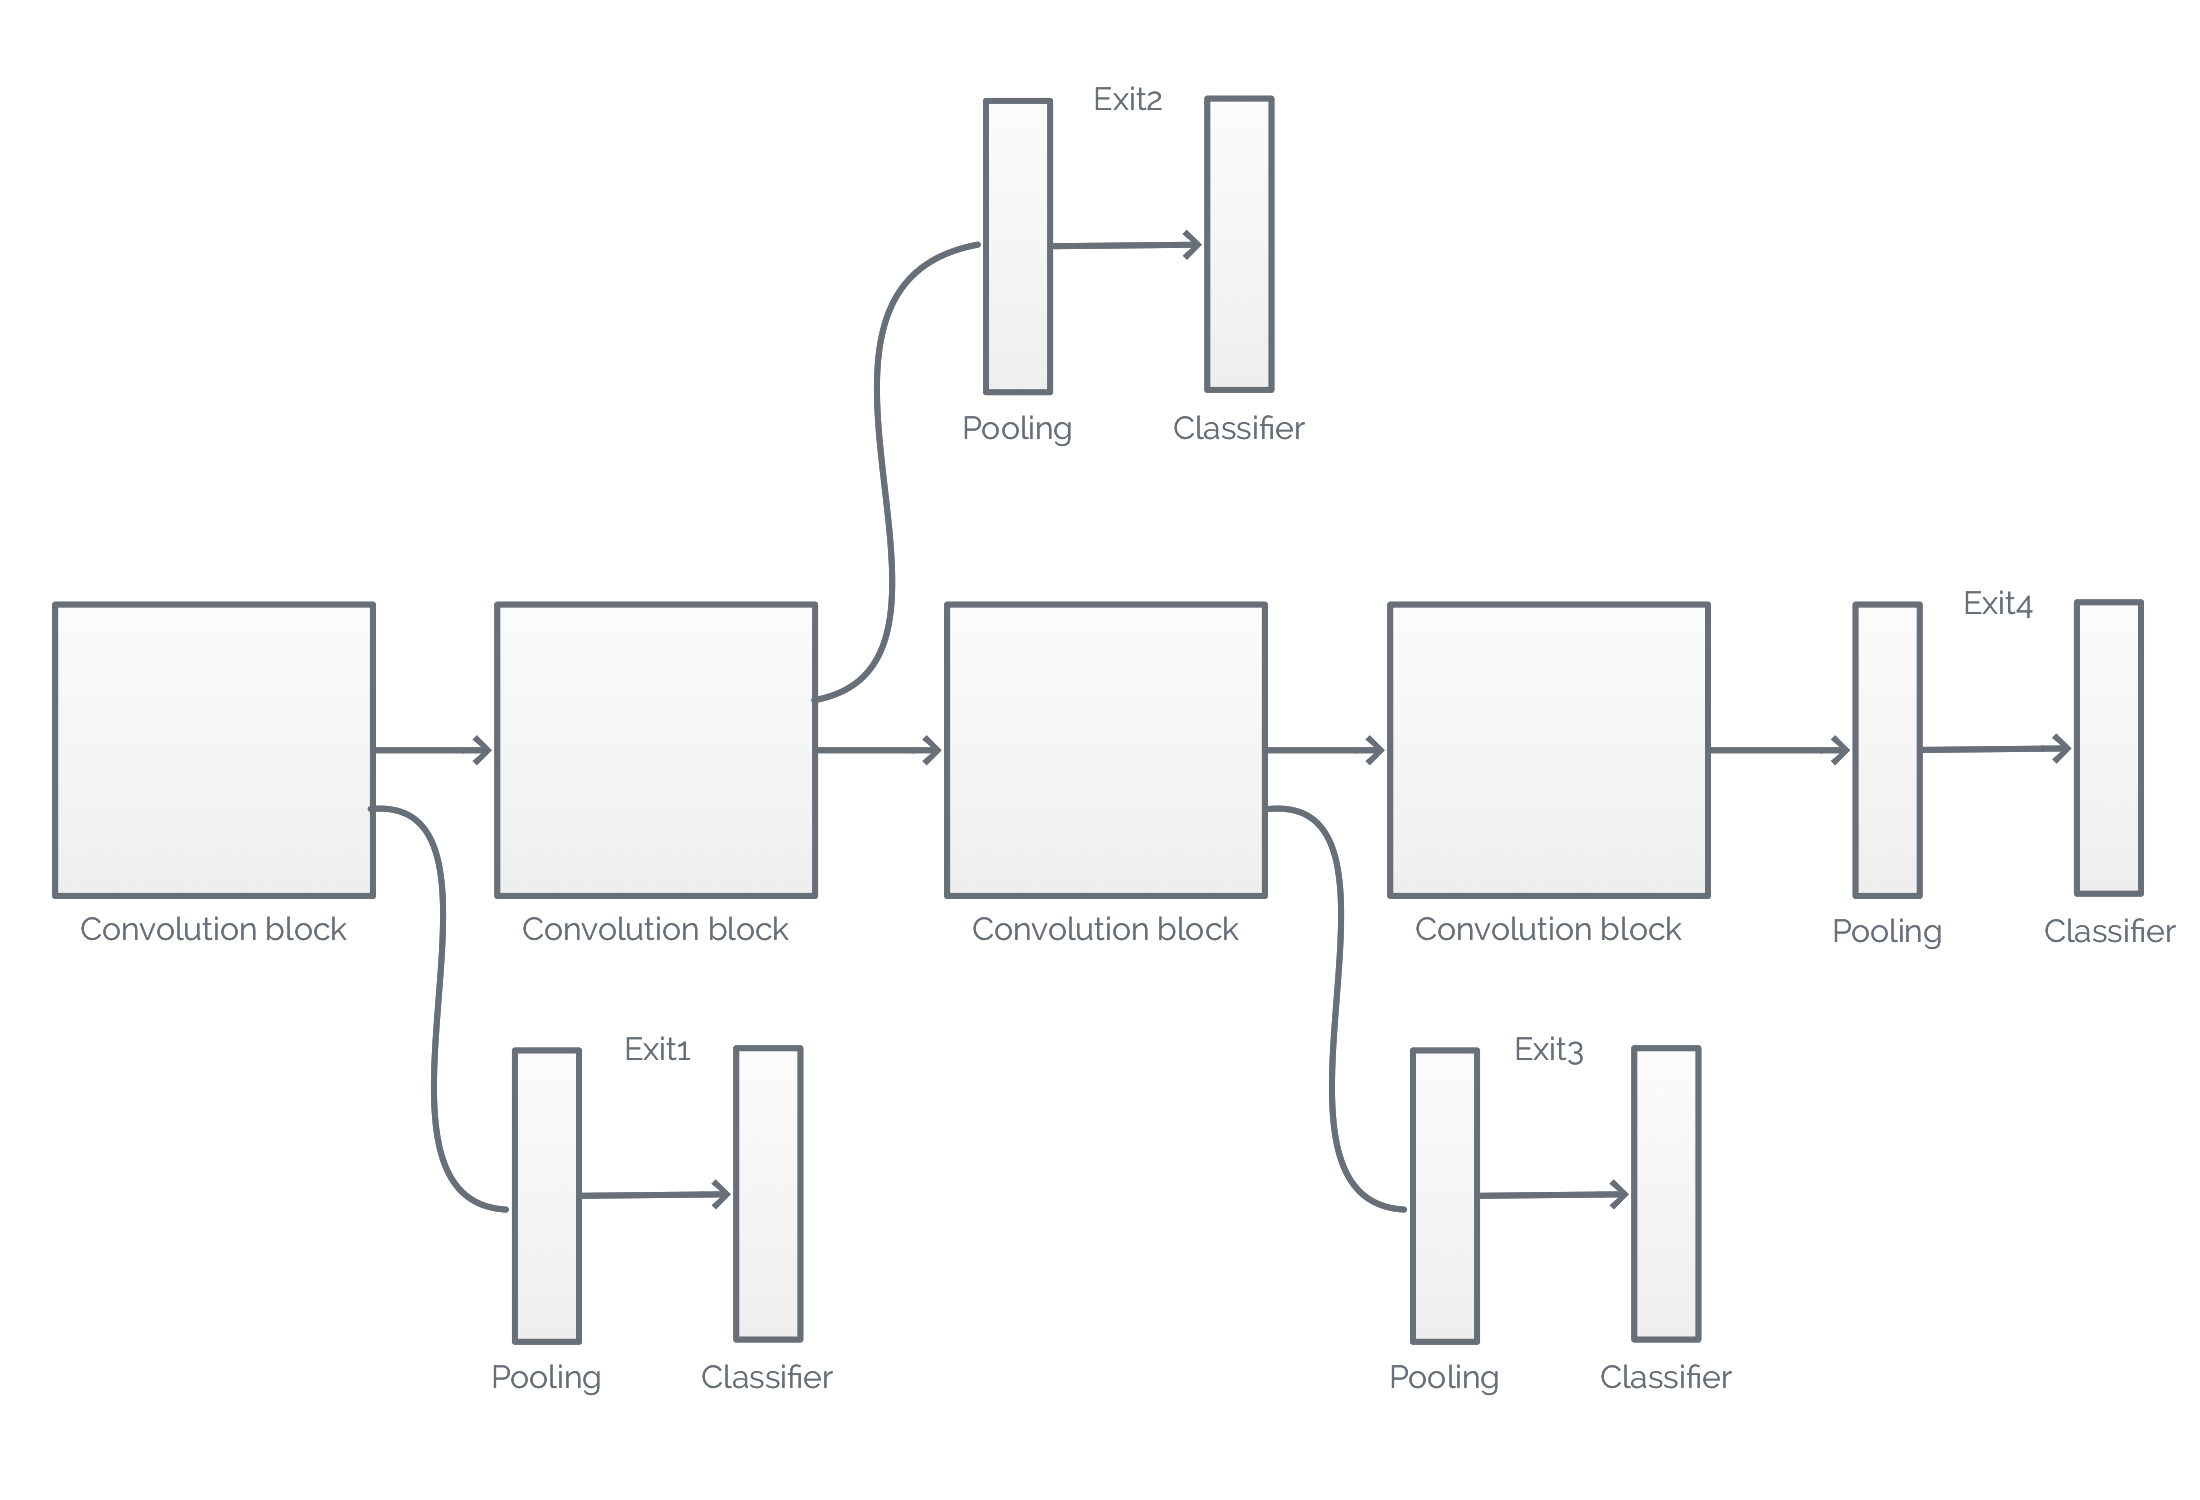
\includegraphics[width=.7\linewidth]{figures/models/branchy}
		\captionof{figure}[Early Exit Architecture]{Early Exit Architecture}
		\label{fig:branchynet}
	\end{minipage}

	Our work is based on standalone early exit \gls{dnn}s. Early exit is elaborated upon in section \ref{sec:ee-branchy-vs-cascaded}.
	
	\item[Model Layer Skipping] Other approaches to reduce inference time of \gls{dnn}s involve mechanism for skipping certain layers. SkipNet \cite{wang_skipnet:_2017} is a framework for adding dynamic decision for layer skipping. 
	
	\begin{minipage}[t]{\linewidth}    
		\centering                          
		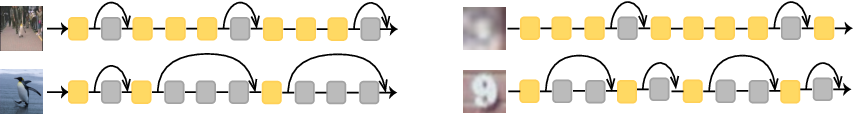
\includegraphics[width=.8\linewidth]{figures/models/skipnet}
		\captionof{figure}[SkipNet]{SkipNet: Source \citetitle{wang_skipnet:_2017} \cite{wang_skipnet:_2017}}
	\end{minipage}
	
	The framework adds complexity to the model by introducing skipping gates between intermediate layers of the network. SkipNet is trained using a hybrid of supervised- and reinforcement learning. The classification is learnt as a usual supervised problem using labeled data. The skipping policies are learnt using reinforcement learning by rewarding skipping decisions, that have little impact on classification accuracy. The work shows, that only a small fraction of inputs actually require these extremely deep models, thus SkipNet is able to reduce the computational cost by 30\% of \gls{resnet}101 on \gls{ilsvrc2012}. 
	
	BlockDrop \cite{wu_blockdrop:_2017} is another approach to learn skipping policies. However, instead of adding intermediate skipping gates for dynamic local decisions, BlockDrop trains a global policy network, that selectively chooses which model depth to use. BlockDrop is in fact a learned model selection framework, where the selection of models is not based on a confidence output of a smaller model, but on a \gls{dnn} trained to predict the complexity of an input sample. 
	
	
	\begin{minipage}[t]{\linewidth}    
		\centering
		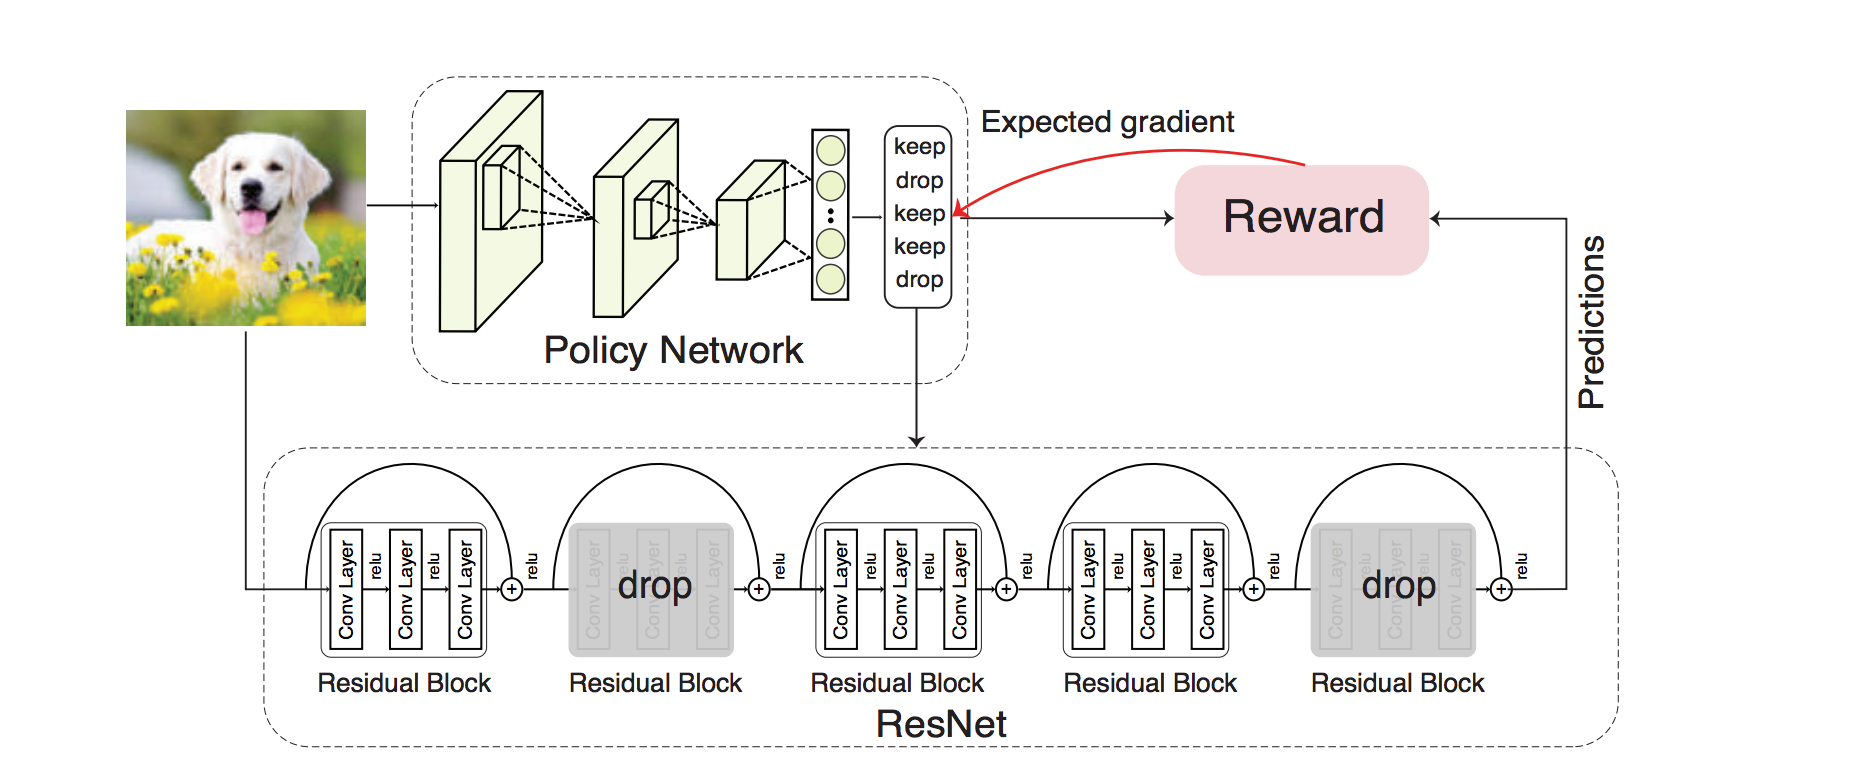
\includegraphics[width=\linewidth]{figures/models/blockdrop}
		\captionof{figure}[BlockDrop]{BlockDrop: Source \citetitle{wu_blockdrop:_2017} \cite{wu_blockdrop:_2017}}
	\end{minipage}
	
	The policy network is similarly trained using reinforcement learning. The training shows, which classes are easy and which are hard. SkipNet and BlockDrop could both be used in an edge-device mode such as a Big/Little \cite{park_big/little_2015} setup. Particularly BlockDrop where the inexpensive policy network is run by an end device to selective choose among a smaller model on-device or a larger model on an edge server to avoid wasteful executions.
%Although Big/Little \gls{dnn} obtain good results on energy savings and inference latency, other approaches such as early exiting, tries to reduce wasted computation of the little \gls{dnn}, by creating multiple exits in an existing model.	


\end{enumdescript}

\subsection{Collaborative Inference}

In this subsection we present efforts at reducing inference time for collaborative architectures. Instead of solely executing a \gls{dnn} in the cloud, edge or on device, the computing resources collaborates to boost inference time. Collaborative inference of a conventional \gls{dnn} is also known as model partitioning. Splitting a model is an inherent nature of sequential \gls{dnn}s. The inference process can be stopped at any layer. The intermediate output after the last executed layer are transferred over the network, and the inference continues at the next layer on an edge server, as shown in figure \ref{fig:offlaoding}.

\begin{minipage}[t]{\linewidth}    
	\centering
	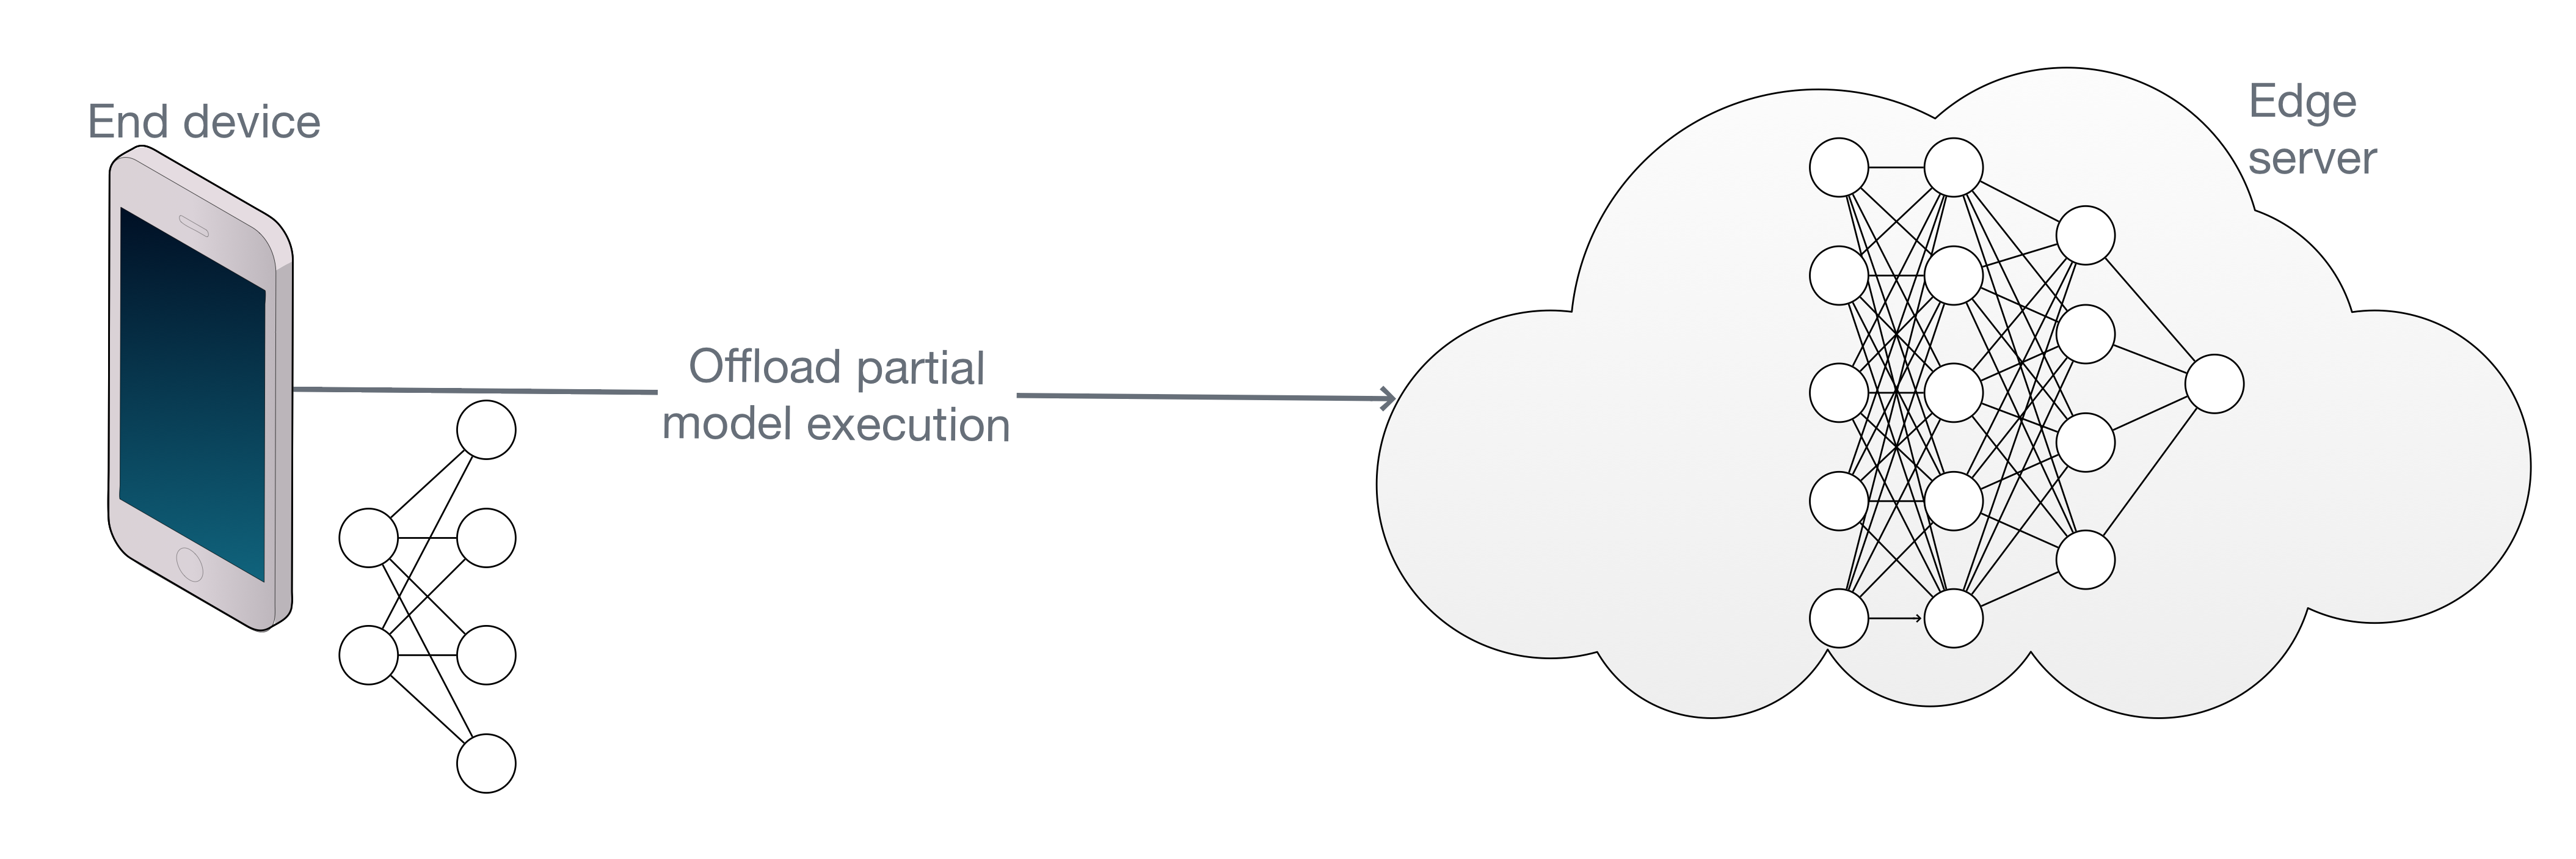
\includegraphics[width=\linewidth]{figures/models/partitioning}
	\captionof{figure}[Model partitioning]{Edge-Device model partitioning run part of the model on-device and offload the rest to edge processing. Network partitioning utilize the assumption, that at some later point in the \gls{dnn} a smaller representation of the data is found, illustrated by the gradually decreasing model layers, to reduce the communication bottleneck. }
	\label{fig:offlaoding}
\end{minipage}

Neurosurgeon \cite{kang_neurosurgeon:_2017} is a lightweight partitioning scheduler, that uses knowledge of the individual layers of the \gls{dnn} to effectively reduce inference latency. Communication delay is the bottleneck in such an offloading application, hence a smaller representation of the input data is needed, however the layers producing a smaller output than the original input, typically lies deep within the network. Neurosurgeon construct regression models for per layer execution time and output data size of the \gls{dnn}. The regression models are used to decide the best partition of the \gls{dnn} based on available communication data rate. The work is based on \gls{ci} setup and shows, that the conventional cloud-only approach is actually insufficient, due to low data rate connections with high variability to cloud data centers and the trend that more mobile device is being equipped with \gls{gpu}s. 



%Since early exiting less computation is wasted, if offloading is necessary after an exit compared to a Big/Little model selection setup. As less computation is needed and a smaller representation of input data can be obtained, thus less data must be offloaded to the edge server.
\begin{enumdescript}
	\item[Feature Compression] 

	% Evidently moving computation to the edge reduces the communication latency. 
	
	Efforts have been made to reduce communication overhead, when splitting \gls{dnn}s to run in a collaborative scheme. One of which is compression of intermediate features before offloading to cloud or edge \cite{choi_deep_2018}. The paper shows, that lossless compression has, no impact on accuracy. However, bit saving is also rather limited. Lossy compression, on the other hand, results in 70\% bit savings, but also have negative impact of model accuracy. To compensate, a compression aware training have been proposed. The follow up paper \cite{choi_near-lossless_2018} propose a novel compression technique, especially designed for deep features i.e. the output of an intermediate \gls{dnn} layers, and with significantly higher bit savings compared to conventional image compression algorithms such as JPEG. Alternatively, methods such as \gls{bottlenet} \cite{eshratifar_bottlenet:_2019}  proposes novel \gls{dnn} module, that creates a low dimensional representation of the output features, able to be restored to original dimensionality. 
	
	
%	\begin{minipage}[t]{\linewidth}    
%		\centering
%		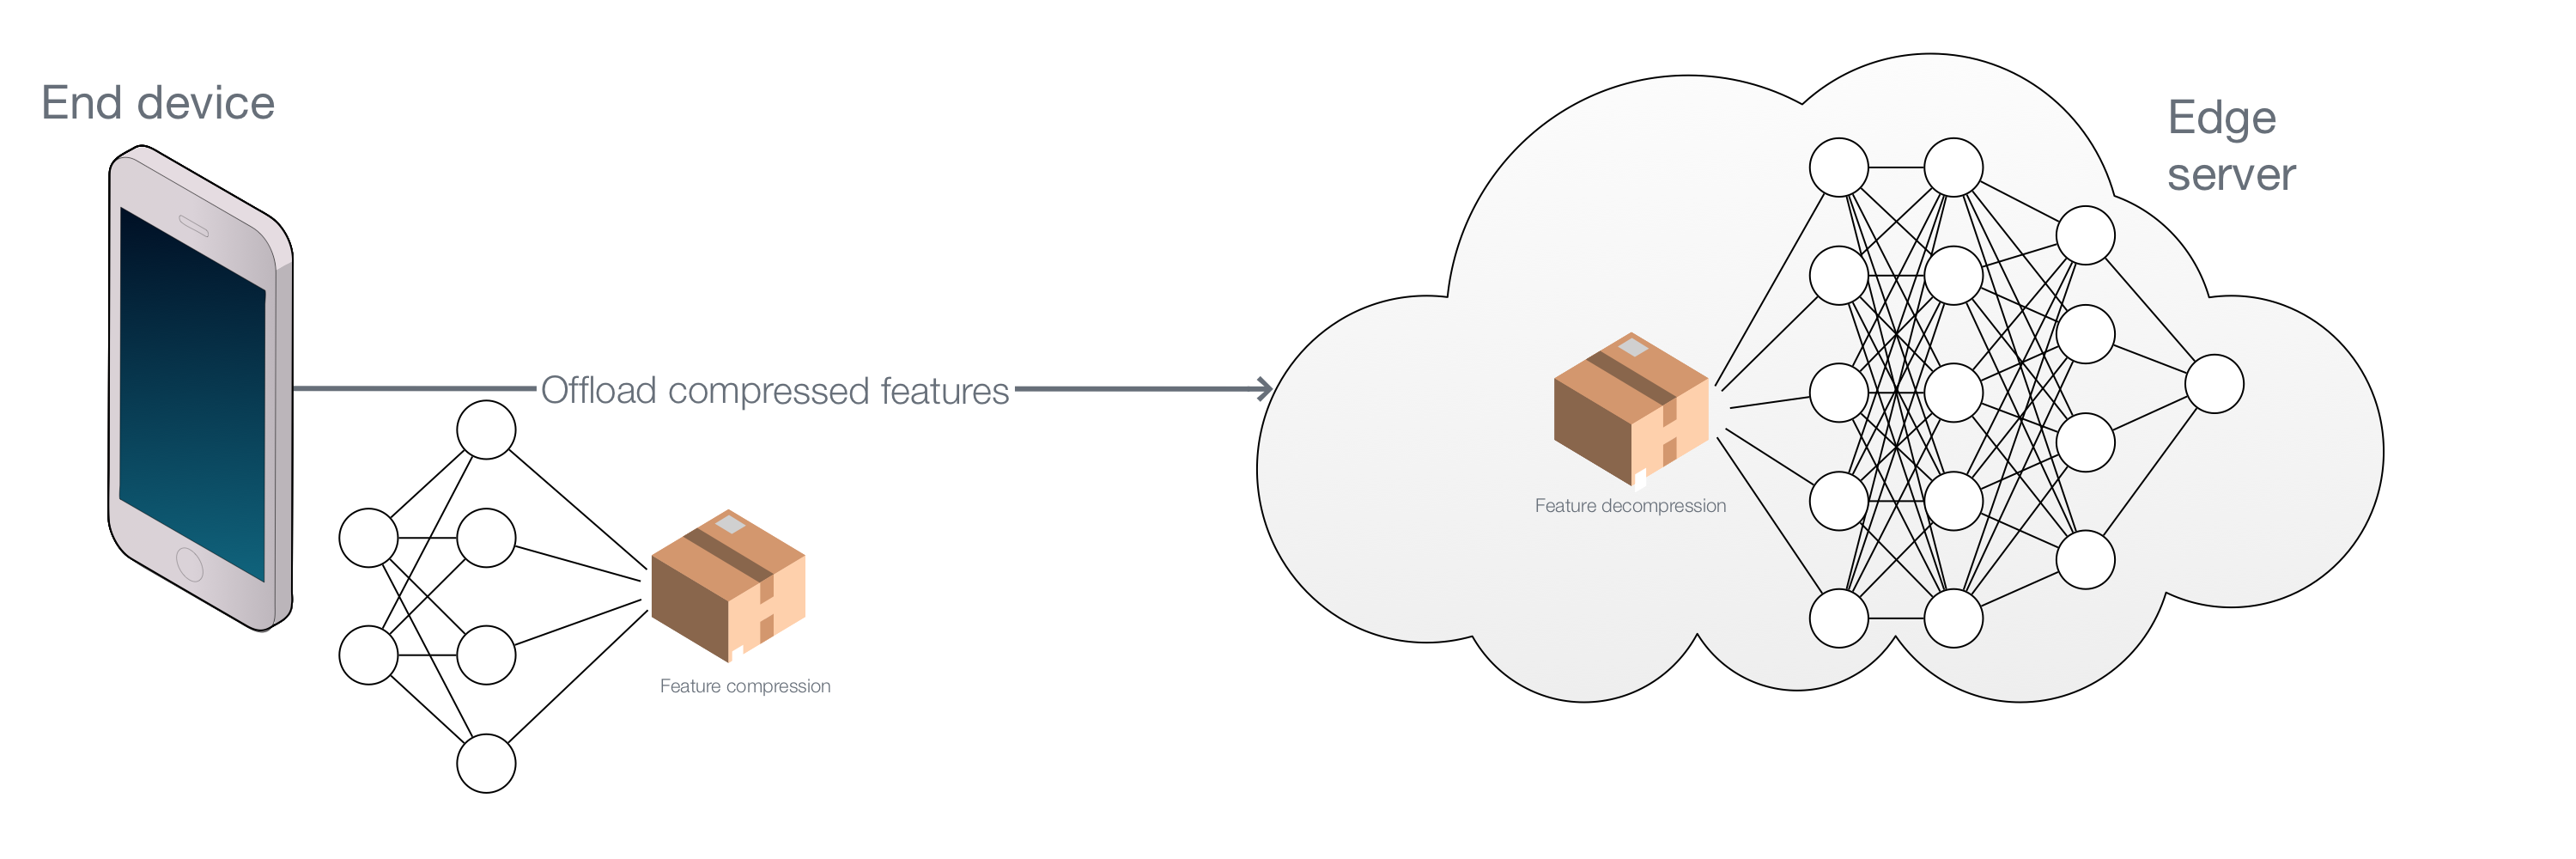
\includegraphics[width=\linewidth]{figures/models/compressed}
%		\captionof{figure}[Feature compression]{Feature compression}
%	\end{minipage}
	
%	\gls{bottlenet} is a novel neural network module.
	Client-side \gls{bottlenet} implements of a reduction unit and a compressor unit. The reduction unit creates a smaller representation of intermediate features by applying spatial- and channel-wise convolution. The compressor uses lossy JPEG compression and sends the data to the server. Server-side it implements a decompressor unit and restoration unit. The server decompresses the received data and the restoration unit restores the intermediate feature using channel- and spatial-wise deconvolution, to get the required input size for the next layer in the \gls{dnn}.
	
	\begin{minipage}[t]{\linewidth}
		\centering
		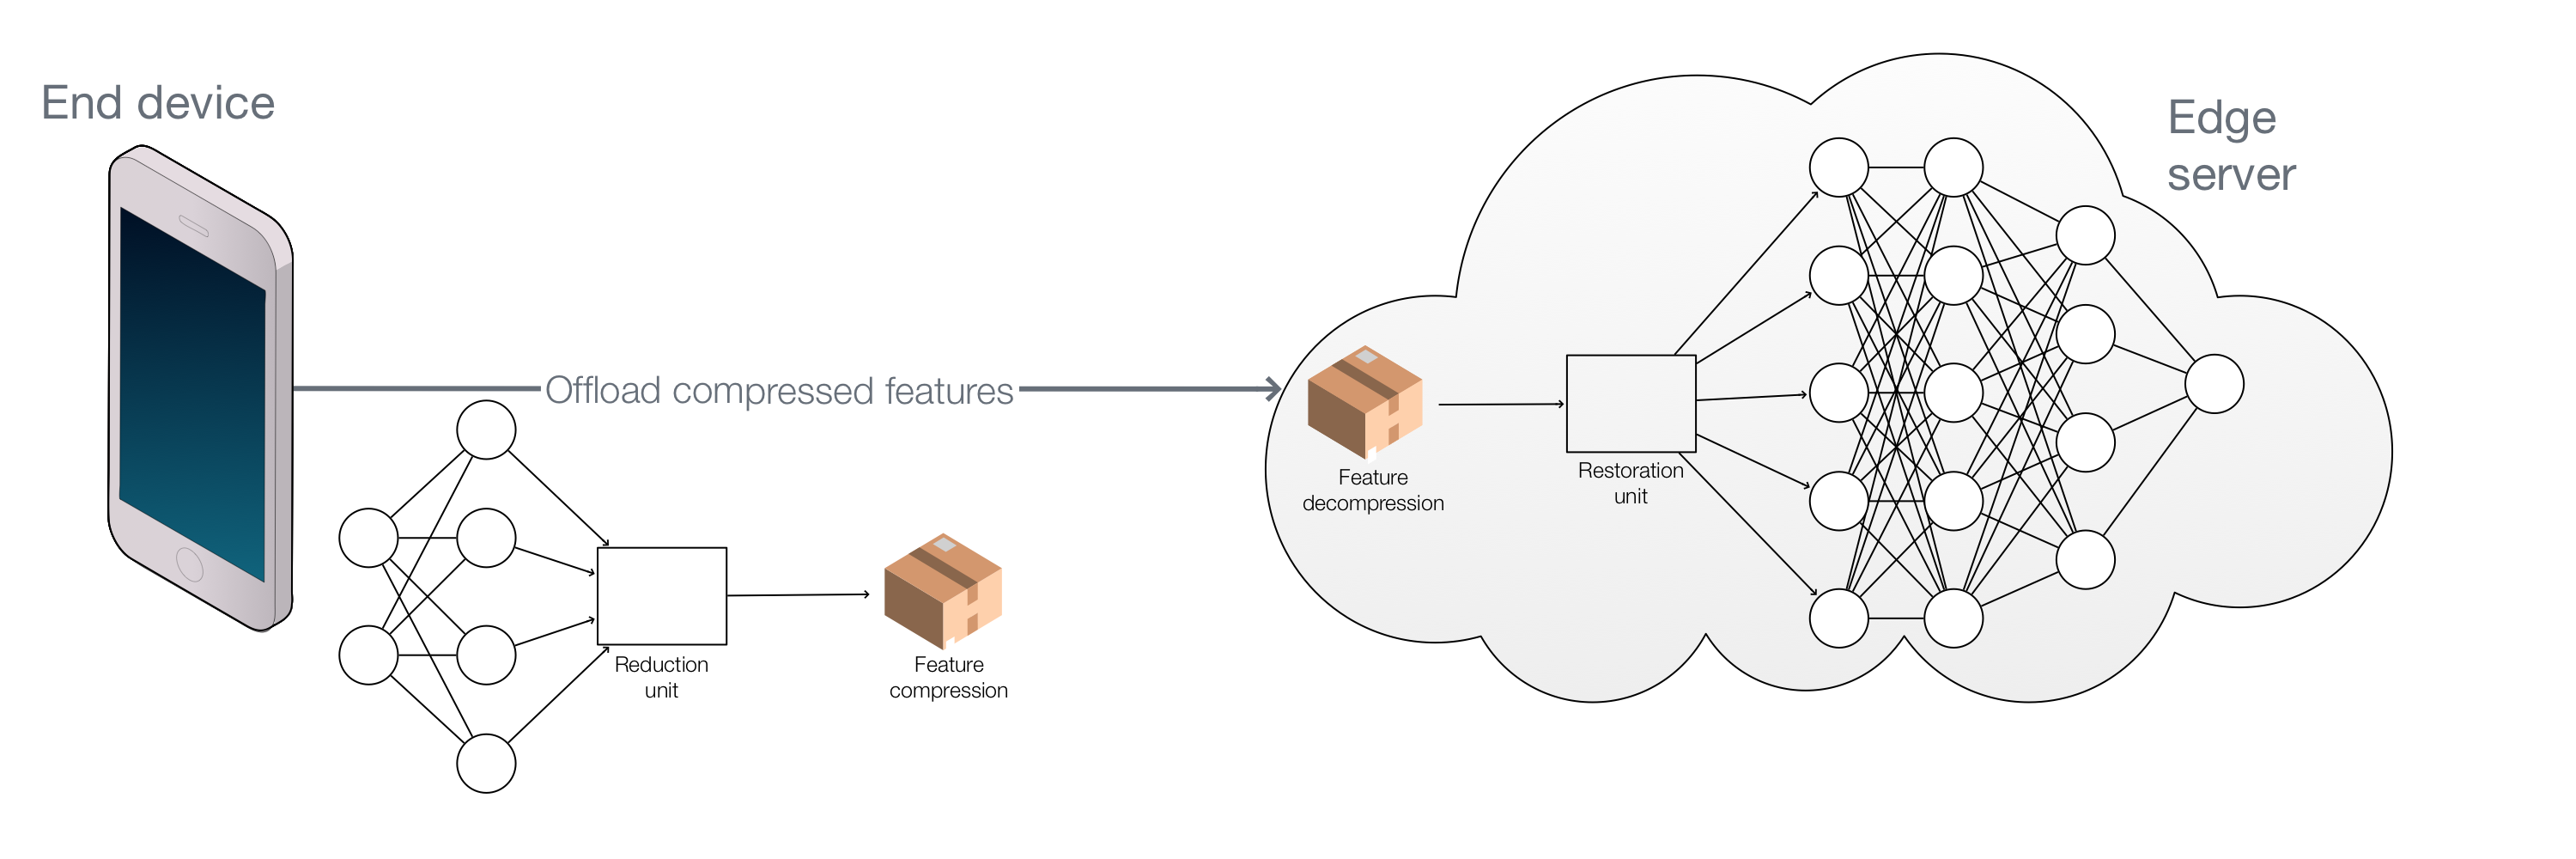
\includegraphics[width=.8\linewidth]{figures/models/bottlenet}
		\captionof{figure}[BottleNet Unit]{BottleNet Unit}
	\end{minipage}

	\gls{bottlenet} is able to achieve 84$\times$ bit savings compared to cloud-only approach with less than 2\% degradation of accuracy caused by lossy compression with compression-aware training. Under good networking condition, the evaluation of \gls{bottlenet} shows, that the best split is after the first convolutional block, as a smaller representation of the input can already be found using reduction and compression. Compared to cloud-only approach using WiFi a 8$\times$ speed up is found. 
	
	\item[Distributed Exits] Cascading neural network have been followed up in \cite{leroux_cascading_2017}. The paper uses the early exiting model, to distribute the \gls{dnn} between end devices, edge and cloud. Figure \ref{fig:early-exit-colab} illustrates a partitioned early exit \gls{dnn} for collaborative edge. 
	
	\begin{minipage}[t]{\linewidth}
		\centering
		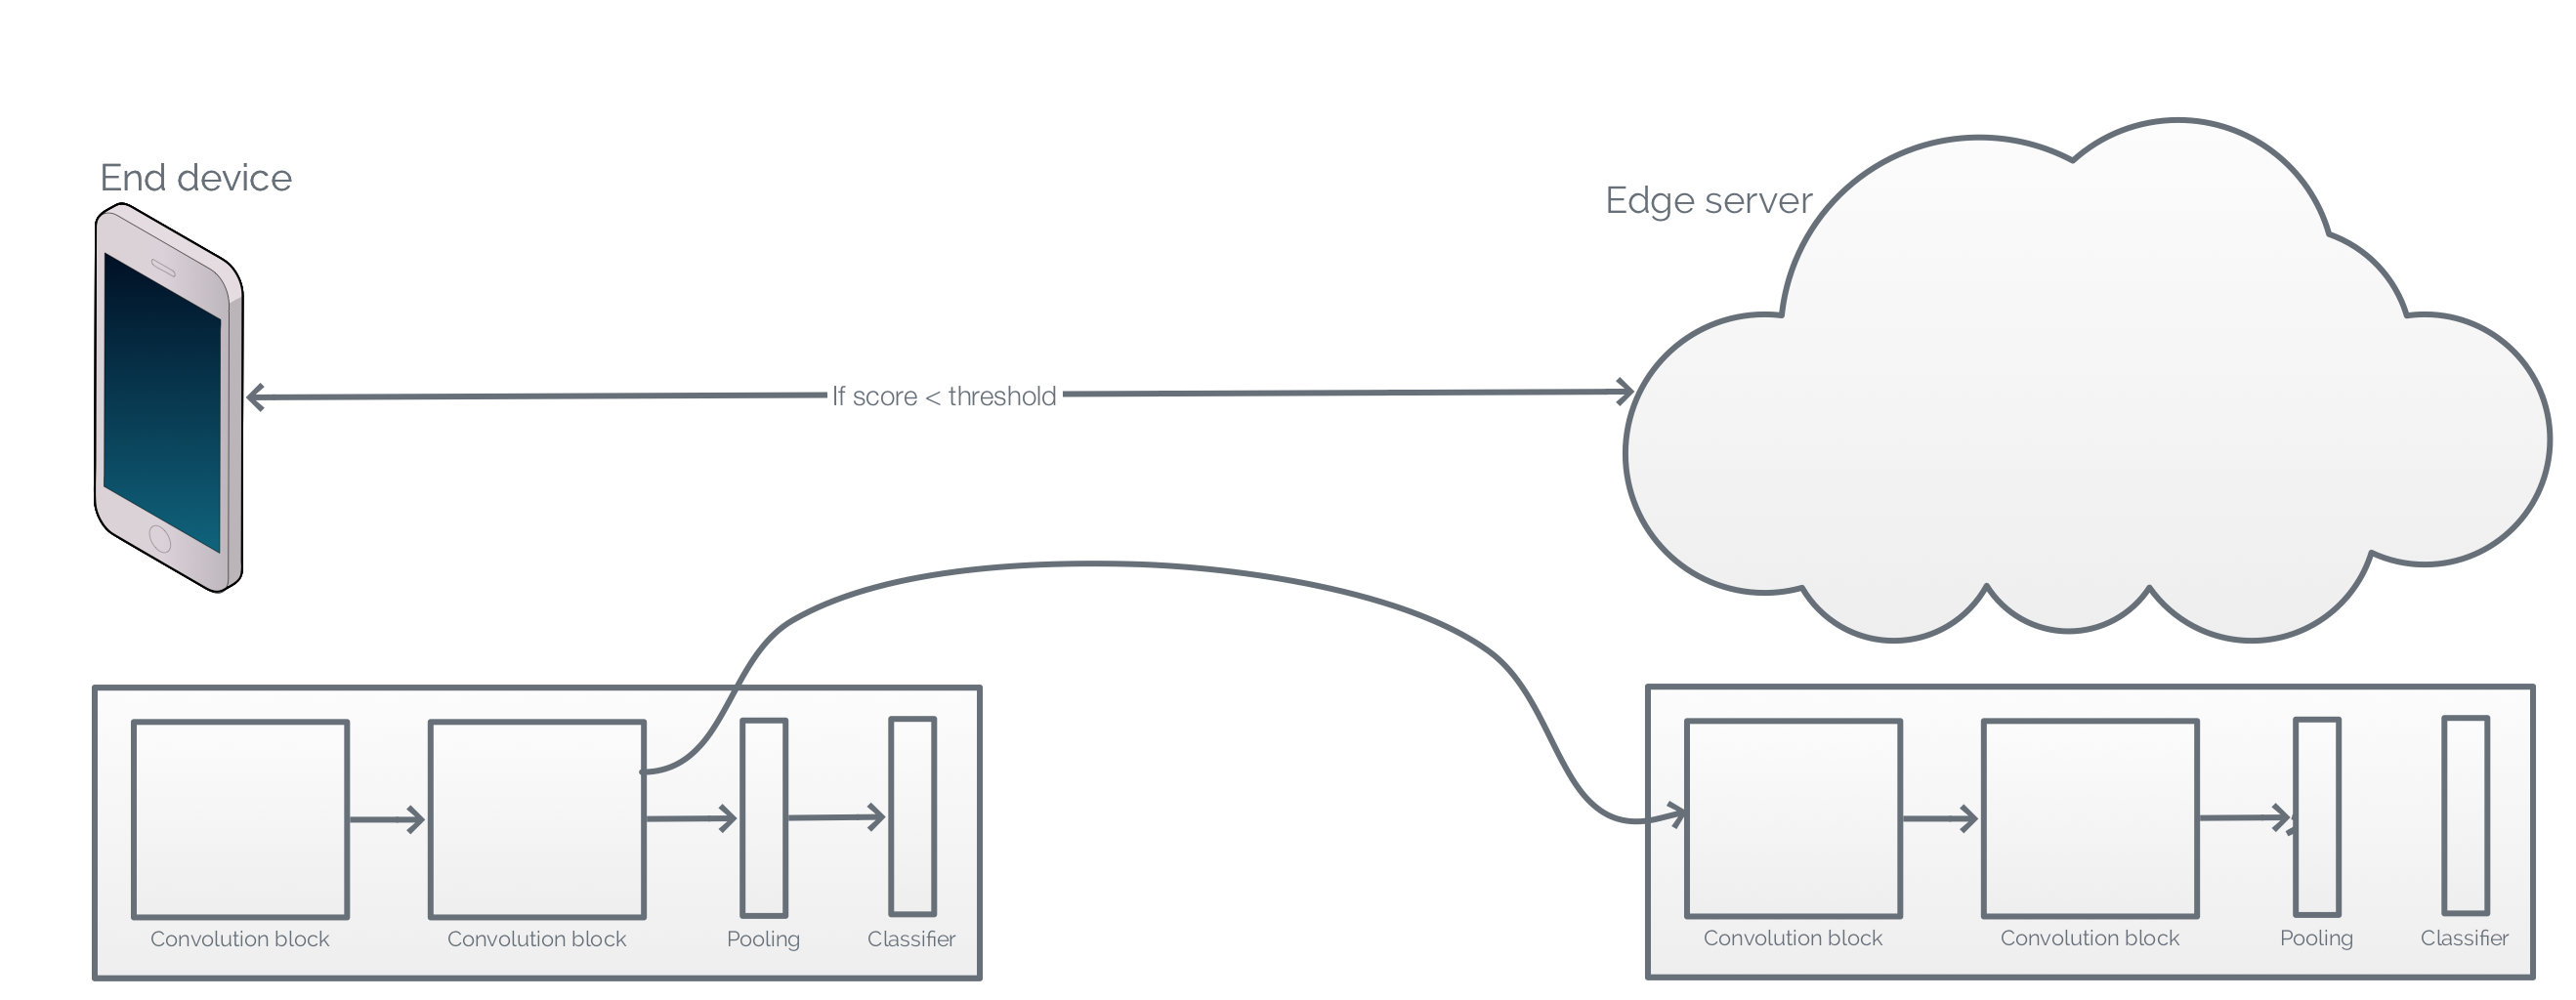
\includegraphics[width=\linewidth]{figures/models/cascaded}
		\captionof{figure}[Cascaded \gls{dnn} over a computing hierarchy]{Cascaded \gls{dnn} over a computing hierarchy}
		\label{fig:early-exit-colab}
	\end{minipage}
	The model is distributed in a manner, where one or more exits are processed by the end device, and one or more exits on the edge server. To save communication efforts the process is terminated, if a satisfying prediction is obtained locally. Nonetheless, model partitioning introduces communication delay to the inference task, that most be accounted for e.g. using one of the method for feature compression.
	
	\gls{ddnn} \cite{teerapittayanon_distributed_2017} extends the idea of partitioning early exit models between a device, edge and cloud hierarchy. They propose a framework to allow geographically distributed end devices to collaborative solve a \gls{dnn} inference task in the hierarchy. The intermediate output from the geographically distributed end-devices are aggregated for a local prediction. Based on the score, the inference is exited locally or sensor fusion of the intermediate features are performed by the \gls{dnn} at a higher peer in the hierarchy. Using early exit model in this fashion, does not only show improvement for early exits but also the final prediction. Additionally, \gls{ddnn} offers benefits from distributed computing to provide fault tolerance, when some local \gls{dnn} comes with a bad, or a missed prediction. \gls{ddnn} have been proposed for Industry 4.0 to solve autonomous defect detection in \cite{li_deep_2018}. 
	
	The cascaded network is used to handle the latency-accuracy trade-off for mission-critical application with a predefined deadline in \cite{li_edge_2018}.  Edgent \cite{li_edge_2018} is built on top of the \gls{branchynet} framework. Edgent is an optimization engine based on a deadline, a regression model of inference time of each layer, and the observed available bandwidth between end device and edge server. Edgent makes a decision, to right-size the model by a selection of an optimal exit point, and to partition the model for collaboratively inference on end device and edge by selecting a partitioning point. Edgent have shown to be able to meet more stringent deadlines, than running solely \gls{branchynet} on device or edge.
\end{enumdescript}

\subsection{Distributed Inference}

\todo{Ask Qi if should be removed}
Distributed inference is similar to collaborative edge. However, instead of partitioning the model in the depth axis i.e. between two layers, as for collaborative inference. Distributed inference seeks to partition the task in the input axis i.e. let multiple peers collaborate to solve single layers. \gls{modnn} \cite{mao_modnn:_2017} is a framework to distribute the computing of the input to multiple worker nodes. Distributing computation input-wise can result in a higher degree of data dependence, and lead to more a higher degree of communication between workers. \gls{modnn} show improvement of computing a \gls{dnn} inference on multiple mobile devices connected on a WLAN, compared to standalone inference on a single mobile device. DeepThings \cite{zhao_deepthings:_2018} is a framework intended for constraint \gls{iot} devices to distribute computation. In DeepThings, they take advantage of local region dependency in layers, that can be split into multiple tasks and that the dependency across layers into large tasks. In this manner, they actually split the network layers horizontally but stack the work vertically i.e. just as regularly \gls{dnn}s.